\begin{document}

\chapter{Introduction}

One of the biggest challenge of mobile development today resides in the high fragmentation of mobile platforms \cite{MobileDevChallenges} with developers building the same app over multiple platforms. A popular solution is cross-platform development, that is using a framework capable of using the same code for multiple platform builds. However, such cross-platform development does not concern web applications that developers still have to develop separately from mobile applications. To answer this problem, Google introduced in 2015 the concept of \textit{Progressive Web Apps} \cite{PWA_intro}, a term first coined by designer Frances Berriman and Google Chrome  developer Alex Russel \cite{PWA_blog} \cite{PWApossibleUnifer}.
This section will introduce the concept of Progressive Web Apps and the objective of this paper.


\section{Research questions}

Due to its cross-platform capabilities, Progressive Web Apps seems like a promising alternative to native development. However, this shouldn't come at the cost of app performance and user experience, especially in regards to smoothness.
Thus, this paper will aim at answering the question : 
\begin{center}
    \textit{Can Progressive Web Apps be as smooth as Mobile Applications ?}
\end{center}
Which raises the following sub-questions: 
\begin{enumerate}
    \item What metrics are relevant to compare the smoothness of Mobile and Progressive Web Apps?
    \item What tools are available to measure those metrics ?
\end{enumerate}

\iffalse
Due to its cross-platform capabilities, Progressive Web Apps seems like a promising alternative to native development. However, this shouldn't come at the cost of app performance and user experience, especially in regards to smoothness.
Thus, this paper will aim at answering the question : 
\begin{center}
    \textit{Are Progressive Web Apps as performant as Mobile Applications in terms of smoothness?}
\end{center}
Which can be divided into the sub-questions: 
\begin{enumerate}
    \item How can we compare the smoothness of Progressive Web Apps and Mobile Applications ?
    \item With the metrics identified previously, are Progressive Web Apps as smooth as Mobile Applications ?
    \item How many resources are used to render a smooth application ?
\end{enumerate}
\fi

\iffalse
Primary research question : 
\newline \textit{How efficient can Progressive Web Apps be compared to a Native Android Application?}
\newline
Secondary Research questions :
\\1. \textit{How can we compare Progressive Web Apps and Mobile Apps ?}
\newline \indent
1.1 \textit{What metrics are relevant to compare Progressive Web Apps and Mobile Apps ?}
\newline \indent  
1.2 \textit{What tools are available to measure those metrics?}
\newline
\\2. \textit{Are Progressive Web Apps more efficient than Mobile Apps with regards to the first question?}
\fi

Due to its cross-platform capability, Progressive Web Apps seems like a promising alternative to native development. However, this shouldn't come at the cost of app performance and user experience, especially in terms of the app smoothness and rendering capacity.
Thus, this paper will aim at answering the question : 
\begin{center}
    \textit{Are Progressive Web Apps more performant than Mobile Apps in terms of rendering capacity ?}
\end{center}
Which can be divided into the following sub-questions: 
\begin{enumerate}
    \item How can we compare Progressive Web Apps with Mobile Applications?
    \item What tools are available to measure the relevant metrics ?
\end{enumerate}

\chapter{Background}
%This chapter introduces the terminology and concepts used this study, as well as previous research done on Progressive Web Apps and available tools to measure Android apps and PWA's performance. 

\section{Mobile Applications}
\subsection{Development}

React Native, Ionic and PhoneGap are one of the most popular frameworks used today \cite{CrossPlatform_study}.

%The smoothness performance can refer to the result display on the screen, and its efficiency in resource consumption. the research question will be divided into the following sub-questions:


%\paragraph{R2:}
%With the metrics identified previously, are Progressive Web Apps as smooth as Mobile Applications?
%\paragraph{R3:}
%How much resources are used to render a smooth application?
%\begin{enumerate}
  %  \item How can we compare the smoothness of Progressive Web Apps and Mobile Applications?
 %   \item With the metrics identified previously, are Progressive Web Apps as smooth as Mobile Applications?
%    \item How much resources are used to render a smooth application?
%\end{enumerate}


%\section{Limitations}

%\todo[inline]{Maybe is a good idea to move to the conclusion}

%Every research paper comes with its limitation, and this work is no exception. 
%At the time of writing, Progressive Web Apps are not fully supported on iOS \cite{BackgroundSync_support} \cite{Manifest_support}. Thus, this work will focus on comparing PWA and traditional mobile applications only on Android. 
%Moreover, according to Statcounter \cite{Browser_data} which compiles data from more than 10 billion page views per month, the browser used the most on mobile is Google Chrome with more than 60\% usage followed by Safari with 26\% and other browsers at less than 10\%. 
%Considering the overwhelming usage of Google Chrome on Android devices, this paper will focus on PWA's performance with Google Chrome. 


\section{Progressive Web Apps}
\subsection{Academic research}

Since June 2019, more than half of Web traffic comes from mobile devices. \cite{WebTrafficData}

    \cite{smoothnessQoE} build a model to evaluate the smoothness of smartphones. This model focuses on two major indexes : the maximum frame interval and the total number of frames in different key behavior scenarios (phone calls, browsing the web, playing games, etc). Those frames are defined as the interval of time between user input and response time of several key display events measured with a camera. %To check this frame definition
    
    \cite{PWAbc_responsetime} measured the response time between an Android app and a React PWA when accessing the Camera and Maps. The response time was measured 54 times for each scenario. The results show that Native are faster for accessing the camera, though PWAs are making progress in that regard. However, PWAs are faster regarding geolocation and map rendering.
    
    \cite{YbergViktor2018NPaU} focused on the user experienced of PWAs and measured several performance metrics: load times (Polymer, React, Preact), start-up times (native app, Polymer with and without browser in memory), Lighthouse performance audit (Polymer), list rendering times (PWA). He concluded that PWAs provided a good enough user experience for information access apps, though PWAs are not fully supported on every platform and web browser.
    
    \cite{PWApossibleUnifer}, followed by \cite{Biorn-Hansen2} shows a lack of academic research on the subject. \cite{PWApossibleUnifer} developped three apps using the Hybrid, Interpreted and PWA approach and compared their startup speed, app size and rendering speed. They conclude that PWA have a lot of potential to unify web and mobile development, though some limitations remains (lacking some hardware access, and browser support on some platform).
    
    \cite{Biorn-Hansen2} developed 5 apps: a PWA, a native app written in Kotlin, an Ionic hybrid app, an Interpreted React Native app and a cross-compiled Xamarin app. Again, they measure the app size, the activity launch time and the time from app icon to toolbar rendering. They reconfirmed the potential of PWAs to have an important part in futur Mobile development, depending on iOS support. They are extremely small compared to other apps, and render content fast. Although they lack some hardware access, they are also the only ones testable before install. 
    
    \cite{SW_and_energy} studied the energy impact of service workers on PWAs. Their results showed no significant energy impact from service workers. However, it also showed different energy consumption of each PWAs
    
    \cite{JohannsenFabian2018PWAa} studied how turning a regular web app into a PWA affects the code complexity in Angular. It concluded that the main increasing factor is the understanding of the new concepts behind the service workers, but automated PWA tooling can decrease it.
    
    \cite{Pride_Prejudice} identified several security threats regarding PWAs
    
    \cite{bac_pwa_comparison} found that PWAs had a slower performance than regular web apps (with lighthouse performance metrics)
    
    \cite{PWA_UX_comparison_study} conducted an analysis of user experience when interacting with a regular web app, a native Android app and a PWA. The 8 participants had an overall good user experience on every platform.
    
    \cite{bac_pwa_performance} studied loading performance (first paint, etc) of PWA in comparison to Apache Cordova app and native android. The results differ between phones %Conclusion noot very clear on this one
    
    \cite{emulating_native_w_crossplatform} compared features from a cross-platform app, a native Android app and a PWA. They were also compared in a qualitative and a qualitative user studies. No real difference was found between the applications. The React Native app performed a little better on the quantitative study, and the PWA performed a little better on the qualitative study.
    
    \cite{PWADatabase} compare performance of same app developed multiple times with different parameters (framework, service-worker, optimization, etc)
    
    \cite{PWAapplicability} compared the same app developed 4 times : a) as a native iOS, b) a native Android, c) a web app and d) a pwa in regards to First Paint and Energy consumption. Regarding the First Paint metric, the PWA performed better against the web app and the native Android app. The difference with iOS might be because of the incomplete support of PWA on iOS. As for energy consumption, PWA seemed to consume less energy, but the number of experiments was not enough to really confirm that.
    
    \iffalse
\paragraph{}
When studying performance, a large portion of the researched papers focused on the app start-up times. They measured either the total launch time\cite{YbergViktor2018NPaU} \cite{PWApossibleUnifer} \cite{Biorn-Hansen2}, the time from app-icon to toolbar render \cite{PWApossibleUnifer} \cite{Biorn-Hansen2}, the first paint \cite{bac_pwa_comparison} \cite{bac_pwa_performance} \cite{PWAapplicability} or other metrics related to start up \cite{bac_pwa_performance} \cite{bac_pwa_comparison}.
Their results showed that the launch time was faster for a PWA than a mobile app when the browser was already in memory. The app icon from toolbar render as well as the first paint metrics also showed that PWA was one of the fastest among the apps tested.\newline
Only one study concluded that PWA was slower than a regular web app because of the HTTPS requests \cite{bac_pwa_comparison}. However, the comparison was made between a PWA served over HTTPS and a regular web app served between HTTP. Another study \cite{bac_pwa_performance} which also compared a regular web app and a PWA First Paint time did not find such results. 

\paragraph{}
Two research papers also investigated the energy consumption of PWA, though from a different angle. Malavolta et al.\cite{SW_and_energy} focused on the impact of service workers on PWA's energy consumption and found no significant impact. Kerssens \cite{PWAapplicability} on the other hand measured the average energy consumption when running the app and found PWA consumes slightly less than its native counterpart. 

\paragraph{}
Fransson and Driaguine \cite{PWAbc_responsetime} compared the response time of PWAs and Native Android Applications when accessing the camera en geolocation. The Progressive Webb App was surprisingly faster at using geolocation than its native counterpart. However, the camera was accessed faster from the native app than the PWA.

\paragraph{}
Lee et al. \cite{Pride_Prejudice} explored the security system behind the push notification system for Progressive Web Apps and found several concerning flaws which they reported to the vendors. 

\paragraph{}
Lastly, only two research papers examined the user experience offered by Progressive Web Apps. Cardieri and Zaina \cite{PWA_UX_comparison_study} conducted a qualitative analysis of user experience on three platforms: web mobile, native android and PWA. They concluded that there was no significant difference of user experience between the platforms. Fredrikson \cite{emulating_native_w_crossplatform} also supports this conclusion with a quantitative and a qualitative study comparing user experience with a React Native App, a Native Android App and a Progressive Web App. 
\fi


\section{Profiling tools}

In order to answer the answer the research question, several metrics will be measured across a number of experiments. The most important one is information regarding the frames produced by the application
%, with a target rate of 60 frame per second \citationneeded \todo{Why?}
. Other metrics will be measured to assess the rendering capacity of the applications : the \%CPU usage of the application as well as the memory used by the GPU. This section covers the tools available to automatically collect the data needed as well as the tools chosen for this study.  


\subsection{Android}
However, this tool is not suited for automatic data collection as the results are only available in charts. Moreover, it can have a high overhead \cite{nanoscope} making the collected data less precise.

\paragraph{}
\textbf{Android Debug Bridge} \cite{adb} is a command-line tool used to communicate with an Android device (physical or emulator) from a computer. It can be used to list available devices (command \textit{devices}), forward requests (command \textit{forward} or execute commands on the device (command \textit{shell}). It will be widely used during this study. 

\paragraph{}
\textbf{Dumpsys} \cite{dumpsys} used with \textit{adb shell} provides information about the device's system services. A lot of different services (thus information) is available through this command-line tool, for example the network, the battery usage, input events, \red{etc}. The most interesting services for this study are: \todo{Rephrase} 
\begin{itemize}
    \item \textit{gfxinfo} which provides information regarding the animation such as jank rate (percentage of frames considered janky ie not meeting the 60fps threshold), total number of frames since recording, etc. It can be used with two options : \textit{framestats} which gives additional information about the frame timestamps, and \textit{reset} which reset the information recorded until now. This information is retrieved by Android framework during the application run-time.
    
    \item \textit{cpuinfo} gives the \%CPU usage of each process running during a given interval of time. The system computes this information from the proc/stat/ files (similar to the files of the same name found on Linux systems) and displays it as the percentage of CPU time used over the total CPU time available in one CPU core with a 0.1\% precision. The information is updated whenever the system needs it and  \todo[color=cyan!20]{Do I cite the source code for that ?} \todo{Yes:)} at least every 30min so the output is not always up-to-date.  
    
    \item \textit{meminfo} takes a snapshot of the memory allocation and outputs the data in details. The main field of interested displays by this command is the amount of memory used for graphics buffer queues. Coincidentally, it also checks the information contained by \textit{cpuinfo} is up-to-date. Thus, it is also used in the experiments to update \textit{cpuinfo}
\end{itemize}

\paragraph{}
\textbf{Top} comes from the Linux command-line of the same name, but with limited options. It displays the process activity in real-time (\%CPU, memory used and other). Its source of information is the same as dumpsys. However, the \%CPU displayed is the percentage of CPU time used over the total CPU time available in the device, with a 1\% precision. This makes it less accurate especially for processes that doesn't consume a lot of CPU. Thus, this command-line was discarded in favor of dumpsys.

\paragraph{}
\textbf{Systrace} \cite{systrace} records a device activity during a short period of time and outputs it in the form of an html file. The file can be viewed on Chrome Browser and displays a timeline of events for each threads running during the recording. The events displayed depends on the categories selected when starting the recording. This tool isn't suitable for automated experiments but can be really helpful to understand the cause of a bottleneck or, as it is the case in this study, understand how Android system works.

\paragraph{}
\textbf{Systrace} \cite{systrace} records a device activity during a short period of time and outputs it in the form of an html file. The file can be viewed on Chrome Browser and displays a timeline of events for each threads running during the recording. The events displayed depends on the categories selected when starting the recording. This tool isn't suitable for automated experiments but can be really helpful to understand the cause of a bottleneck or, as it is the case in this study, understand how Android system works.

\paragraph{}
\textbf{Monkeyrunner} \cite{monkeyrunner} is a tool used to interact with an Android device from a Python script. Aside from sending events and executing \textit{adb shell} commands, it can also take screenshots to test the app. This tool was used to automate the experiment and remove the variables introduced by human interaction from the experiments. 

\subsection{Chrome}

As Progressive Web Apps are after all web applications that runs on the browser, many of the tools available depends on the browser running the app. Thus, the tools presented here may only apply to apps running on Chrome.

\paragraph{}
\textbf{Chrome DevTools} is a set of developer tools available in the Chrome Browser in order to inspect a page on the browser (the network, the performance, the memory, the elements, etc). The main tool of interest here is the \textit{Performance} panel \cite{chrome_devtools_perf} which can record certain events during a period of time and display a lot of information from these events. Among the features of interest are : the display of the duration of a frame as well as the CPU time used to compute it, a CPU, an FPS and a memory chart in addition to a timeline of different events recorded.

\paragraph{}
\textbf{Lighthouse} \cite{lighthouse} is an automated  tool used to assess any web page's quality but mainly targeting Progressive Web Apps \cite{PWApossibleUnifer}. It is available from the \textit{Audits} panel on Chrome Devtools and can retrieve a large number of metrics from an automated recording. Those metrics are classified into five different groups: Performance, Accessibility, Best Practices, Search Engine Optomization (SEO) and Progressive Web Apps, and give an overall score from 0 to 100. It was often used in previous research on PWA \cite{}

\section{Rendering pipeline}

\subsection{Android}
Multiple Application Renderers can communicate with SurfaceFlinger at the same time.   When an application needs to display something on the screen, it pushes a 'surface' to a BufferQueue shared with SurfaceFlinger. Every once in a while, usually in synchronization with the screen refresh rate, SurfaceFlinger wakes up and look into the BufferQueues.

\subsection{Chrome}
However, some stages can be skipped depending on the change between two frames.

\section{Problem analysis}
In the light of the background described above, this sections provides additional motivation and limitations for the research questions. 
\paragraph{}
\textbf{Motivation} \newline

Previous research about Progressive Web Apps performance focused mainly on the performance at start-up (loading time, first paint) but none was found that studied the rendering performance during use. To my best knowledge, this research will be the first to do so.

\medskip
\textbf{Limitations} \newline
As stated above, Android applications and Web Applications on Chrome share two components of the display pipeline (SurfaceFlinger and the Hardware Composer) but differ greatly in the Application Renderer. Thus this research will focus on comparing the smoothness of Android applications and Progressive Web Apps in regards to this last component. 

Thus, this paper will analyze smoothness performance of the applications by looking at the average frame duration, as well as CPU and memory used to compare the resources used. 

\iffalse
However, at the time of writing no study was found that examined the rendering performance of Progressive Web Apps. While it is important for the user that the app launches quickly \cite{launch_time}, it is also important that the app remains smooth during the time of use. \newline
Thus, this paper will try to address this issue and study the smoothness of mobile applications and progressive web apps.

Most of the time, the smoothness of an application is associated with its responsiveness i.e. how quickly it can respond to user input.

As defined by nanana, "the principle of smoothness states that objects must change in a continuous fashion, which reduces cognitive load by removing large and unexpected changes in visual information presented to the user". In other words, a smooth animation changes frames and with little changes between them 

In this work, the smoothness of an application is defined as how quickly it can change the display

\paragraph{}
The smoothness of a mobile application is usually evaluated using the frame rate, or FPS for frame rate per second \cite{smoothnessQoE} \todo[inline]{It would be good to clarify what is smoothness and fluidness}. Though as Biørn-Hansen et al. pointed out while studying animation performance in mobile applications, the FPS metric does not give much insight about the fluidness of a user interface where animations run only during a short amount of time and the remaining time is spent idle waiting for new inputs.
\newline
Thus, this paper will analyze the smoothness performance of the applications by looking at the average frame duration, as well as CPU and memory used to compare the resources used. 
\fi

\iffalse
\chapter{Methodology}


The aim of this study is to compare the smoothness of Mobile and Progressive Web Applications, as well as the memory performance and the CPU usage. The main challenge behind this goal is to define a metric able to compare the smoothness of Mobile and Progressive Web App. For this, a model of a frame rendering on Chrome had to be built. This chapter will outline the reasons behind the necessity of this model and the method used to built it. It will also describe the methods and experiments used to evaluate the CPU usage, the memory usage and the smoothness of Mobile and Progressive Apps.

\todo[inline, color=green]{same remark as intro: you need to clarify the relationship between chrome and pWA. Here, you also need to add one sentence to explain what is the model you are talking about (is it an equation, is it a simulator, is it a monitoring tool...)}

\section{Modeling the smoothness of PWA}
\label{method:smoothness}
    
    The smoothness of an application according to Android and Chrome is closely related to the frames displayed by the application\citationneeded. If a frame takes too long to be rendered, the user might notice some stuttering where motions are visibly fragmented or freezing\todo[color=green]{explain stuttering and freezing} where the application halts for a long period of time, resulting in a poorer quality of the User Experience. Thus, comparing the smoothness of Mobile applications and PWA amounts to compare the frame rendering duration\todo[color=green]{frame display duration ?} on Android and the browser, Chrome in this study. Hence, understanding how native Android and Chrome compute frames, for an executing application, is essential. 
    
    \subsection{Rendering a frame in Android}
    
    \paragraph{}
    The main source of graphical information for mobile applications on Android is the service \textit{gfxinfo}. This service outputs several statistics about the application's frames, such as total number of frames rendered, the percentage of janky frames\footnote{Frames that were dropped or delayed} or the different timestamps of the most recent frames. Those timestamps can help developers identify the most time-consuming stage of the rendering pipeline and thus improve the smoothness of their application. \newline
    \indent Another method to follow the computation of a frame on Android is to use the tool Systrace. With the relevant options selected, a developer can visualize the different functions called to compute a frame in a timeline as a flamegraph (see \autoref{fig:android_systrace_zoom}).
    
    \begin{figure}
        \centering
        \includegraphics[width=13cm]{kththesis/Figures/android_systrace_zoom.JPG}
        \caption{Android Systrace - Screenshot}
        \label{fig:android_systrace_zoom}
    \end{figure}
    
    \begin{figure}[!ht]
        \centering
        \includegraphics[width=13cm]{kththesis/Figures/Android_frame_timeline.png}
        \caption{Linking Systrace and frame's timestamps - Screenshot with timestamps added}
        \label{fig:android_frame_timeline}
    \end{figure}
    
    \paragraph{}
    By looking at Android source code\footnote{\url{https://github.com/aosp-mirror/platform_frameworks_base/blob/master/core/java/android/view/Choreographer.java}}, it is possible to link the timestamps gathered by \textit{dumpsys gfxinfo} to the events displayed by Systrace (see \autoref{fig:android_frame_timeline}), giving an overview of the path taken by a frame on Android. \newline
    \indent Every frame starts with a VSYNC signal (first vertical red line in \autoref{fig:android_frame_timeline}), which acts as was presented in \autoref{background:pipeline:android} as a wake-up call for all the components of Android Graphics. The UI thread handles input and animation before measuring and computing the layout of the graphical elements. It updates the frame and hands it to the Renderer thread which issues the drawing commands and pushes the graphic buffer to SurfaceFlinger. To sum up, for Android a frame starts at VSYNC signal and is completed when its graphic buffer is pushed to SurfaceFlinger. We can extract those timestamps to evaluate the smoothness of Android applications.
    
    %\paragraph{}
    %The frame timestamps provided by \textit{gfxinfo} are enough to evaluate the smoothness of an application. From them, we can compute the total frame rendering time from which we ca
    
    \todo[inline, color=green]{Good to conclude with a summary. I suggest to elaborate
- is the process that you described enough to capture a smoothness value for a native app?
- what is this value?
- did you build a tool on top of gfxinfo and systrace to compute the smoothness value?}
    
    \subsection{Modeling a frame in Chrome}
    
    \paragraph{}
    We can see on \autoref{fig:pwa_systrace_zoom} that the frames on Chrome follow a different pipeline and thus remain undetected by Android system. Nonetheless, we can observe common functions in the Systrace flamegraphs of Android applications and Chrome. Both of them use the same function to push a graphic buffer to SurfaceFlinger, and then display a new frame. Thus, if we gather similar timestamps for Chrome's frames than for Android's, it would be possible to compare the smoothness of the applications.
    
    %|t1||t2|...|t3|
    %|e1||e2|...|e3|...|en|
    %\^
    %|
    
    
    \begin{figure}[h]
        \centering
        \includegraphics[width=13cm]{kththesis/Figures/pwa_systrace_zoom.JPG}
        \caption{PWA Systrace - Screenshot}
        \label{fig:pwa_systrace_zoom}
    \end{figure}
    
    Other tools specific to Chrome exist to collect the frames duration of a web application, such as Chrome DevTools performance panel and Telemetry. Nevertheless, the inspection of their source code revealed that they define a frame duration as the interval between two consecutive frames and give no information about the frame rendering time, making those tools useless\todo[color=green]{why useless?} for comparing PWA and Mobile applications on Android.
    
    \paragraph{}
    Comparing the smoothness of Native Android, Hybrid and Progressive Web Applications requires a detailed overview of a frame's rendering pipeline, both on Chrome and Android. The latter provides it with the frame's timestamps gathered by \textit{dumpsys gfxinfo}. No documentation or tool was found to provide a similar overview of a frame's computation on Chrome. Thus, the first step toward comparing the smoothness of Mobile and Progressive Web Apps on Android is to build a model of Chrome's Graphics pipeline, that is identify the workflow of the computation of a frame. 
    
    \paragraph{}
    The key events related to the computation of a frame were identified thanks to Chrome Tracing tool, which can record functions called by Chrome's processes and display them in a flame-chart. With this tool, we can extract a list of events with their timestamps and arguments. Then, we can confront the current empirical model to those events and modify the workflow if it did not correspond to the events recorded. \autoref{fig:model_process} illustrates the iterative process of modeling a frame computation workflow on Chrome.
    
    \paragraph{}
    This workflow was developed alongside a tool, \textit{FrameTracker}, able to track the computation of the frames on Chrome. This tool takes the list of events recorded by Chrome Tracing tool as input, and outputs a list of every frame rendered during the recording with their key timestamps, as modeled by the empirical workflow. 


    \begin{algorithm}
        \TitleOfAlgo{FrameTracker}
        \SetAlgoLined
        %\KwIn{List of events recorded}
        %\KwResult{List of frames with their timestamps }
        %initialization: order events by timestamp\;
        \ForEach{event}{
            \Switch{name of event}{
                \Case{Event1}{
                    startFrame()\;
                }
                \Case{Event2}{
                    updateFrame()\;
                }
                \Case{Event3}{
                    updateFrame()\;
                }
                \Case{EventX}{
                    updateFrame();
                }
            }
        }
        \caption{FrameTracker}
        \label{alg:frametracker}
    \end{algorithm}

    \todo[inline, color=green]{separate the description of the rules you use to monitor and analyze the events from the fact that these rules are implemented as a script in a specific languages environment (i.e., separate the 'what' from the 'how')
Concretely: this paragraph should discuss an algorithm and at the end you can mention that you implemented the algorithm in language YY, because of XXX and this script is publicly available.
For figure 3.4: I suggest to turn it into an Algorithm (in latex)}


    
    \paragraph{}
    To this end, we used Chrome Tracing tool which can record and display many functions called by Chrome's processes. The model was built empirically with an iterative process. The events recorded by Chrome Tracing tool were processed by a script which tracked the frames computed by Chrome as predicted by the model\todo[color=green]{Which model, which prediction?}.  A simplified version of the script is listed on \autoref{alg:frametracker}.
    This script, named \textit{FrameTracker}, goes through the events recorded by Chrome Tracing tool. If the event is the starting event of the frame, it adds a new one to the list. If not, it looks for the corresponding frame in the list of tracked frames and updates its status accordingly. If anything was not as expected \todo[color=green]{Same question: where do these expected values come from} (the status of the corresponding frame, expected child events), an error is raised. The complete script is available on a Git repository\footnote{PWA\_Master\_Thesis repository: \url{https://github.com/camilleFournier/PWA_Master_Thesis}}.
    
    \begin{algorithm}
        \TitleOfAlgo{FrameTracker}
        \SetAlgoLined
        \KwIn{List of events recorded}
        \KwResult{List of frames with their timestamps }
        initialization: order events by timestamp\;
        \ForEach{event}{
            \Switch{name of event}{
                \Case{Event1}{
                    startFrame()\;
                }
                \Case{Event2}{
                    findCorrespondingFrame()\;
                    \eIf{somethingIsWrong()}{
                        print(errors)\;
                    }{
                        updateFrame();
                    }
                }
                \Case{Event3}{
                    findCorrespondingFrame()\;
                    \eIf{somethingIsWrong()}{
                        print(errors)\;
                    }{
                        completeFrame();
                    }
                }
                \Case{Event4}{
                    findCorrespondingFrame()\;
                    \eIf{somethingIsWrong()}{
                        print(errors)\;
                    }{
                        dropFrame();
                    }
                }
            }
        }
        \caption{FrameTracker}
        \label{alg:frametracker}
    \end{algorithm}
    
    \paragraph{}
    If any error was raised, a visualization of the events on Chrome Tracing tool and a revision of the script allowed either to fix a bug in the script or to change the model according to the events observed. \newline
    The model was first built with a single benchmark application with limited interactions. It was then confronted with 10 traces of 8 different PWAs from the Github repositories pwarocks\footnote{\url{https://github.com/pwarocks/pwa.rocks}} and awesome-pwa\footnote{\url{https://github.com/hemanth/awesome-pwa}} to include a wider range of interactions. This confrontation was done 3 times each, with new PWAs until no significant errors remained.
    
    Those errors were:
    \begin{itemize}
        \item \textbf{Edge effects}: the start and end of a recording can happen anywhere on a frame's timeline. Some events, which require previous events or child events according to the model can raise an error at the start or the end of recording. Those errors are kept to a minimum, but can still happen as the recording does not always start or end at the same time for all threads. They do not invalidate the model.
        \item \textbf{Additional surface}: as it will be explained in more details later, every frame rendered is actually composed of aggregated surfaces. Each iframe or video embedded in the PWA adds a surface and make it more difficult to follow the frames. As this project is limited to simple apps with no videos or third-party advertisement, those errors are ignored. They do not invalidate the model.
        \item \textbf{Bugs}: those errors are not explained by the model. However, they are varied and extremely scarce (1 error over 5 000 frames computed) and are not considered statistically significant.
    \end{itemize}
    
%\todo[inline, color=green!40]{Add a conclusion that summarizes how you will compute and compare the smoothness of a PWA and a mobile app}
With this model\todo[inline, color=green]{don't understand what the model is, maybe add a definition} which we will present in the next chapter, we were able to define a metric able to compare the smoothness of Mobile and Progressive Web Apps on Android. This metric is the frame duration, defined as the time span from the start of the computation of the frame until it is passed on to SurfaceFlinger and the Hardware Composer to be displayed on the screen.

\section{Study Subjects}

This section describes how the experiments used to answer the research questions were designed and conducted. Firstly, the use of Android emulators instead of physical devices is considered. Then, the benchmark applications and the protocol used for the experiments are described.

\subsection{Devices}
\label{method:emulators}

Since emulators can provide easy access to a large range of Android devices, their use was considered for the final experiments. The CPU, of which the usage is a key metrics used to evaluate the performance of the applications, is a hardware difficult to emulate \cite{cpu_emulator}. Thus, it is important to test the emulators against a physical device before using them in CPU-related experiments.

As was presented in the background, only a few Android emulators try to simulate accurately the hardware capabilities of the emulated device \todo[color=green]{What does that mean?} and not improve them. Only 3 were identified and tested: Android Emulator, Genymotion and Visual Studio Android Emulator. As was explained previously, the metrics used to compare the performance of the emulators were the CPU usage using \textit{dumpsys cpuinfo}, the total RAM used using \textit{dumpsys meminfo} and the percentage of janky frames using \textit{dumpsys gfxinfo}. The measures were taken while the devices ran the same application that changed a text every few milliseconds. No human interaction was necessary. The results presented in \autoref{tab:emulators_test} are the average of 110 measurements.

\begin{table}[!ht]
    \resizebox{\textwidth}{!}{
    %\centering
    \begin{tabular}{|m{2,5cm}|m{2cm}|m{2cm}|m{2cm}||m{2cm}|m{2,5cm}|}
        \hline
         & \multicolumn{3}{c||}{Samsung S6 (API 7.0)} & \multicolumn{2}{|c|}{Samsung S5 (API 5.0)}  \\
         \hline
         Metrics & Physical device & Genymotion & Android Emulator & Physical device & Visual Studio Emulator \\
         \hline
         CPU Usage (\%) & 72 & 29 & 18 & 48 & 16 \\
         \hline
         RAM (KB) & 72 080 & 24 243 & 17 499 & 56 813 & 16 992 \\
         \hline
         Janky frames (\%) & 13 & 46 & 6 & 3 & 98 \\
         \hline
    \end{tabular}
    }
    \caption{Emulators Tests}
    \label{tab:emulators_test}
\end{table}

\paragraph{}
The results between the physical devices and the emulators are too different to be used in future experiments. Thus, only the available Android smartphones will be used for this project: Samsung S6 (Android version 7.0), Samsung S5 (Android version 5.0) and Samsung Galaxy S (Android version 4.2)


\subsection{Benchmark applications}

A total of 3 benchmark applications were developed for this project: a Native Android app, a Hybrid app using React Native and a PWA using ReactJS. The frameworks React Native and ReactJS were chosen for the Hybrid and PWA because of their popularity and their similarity. Their common library 'react' and common architecture logic reduce the performance difference that can be introduced by the use of different frameworks.

\paragraph{}
Because of the empirical model and the smoothness metric found in \autoref{results:chrome_model} and \autoref{results:metric} all the applications contain the same features: a Clicking screen where the user can change the content by clicking on the screen, a Scrolling screen where the user can scroll the page to see all the content available and a Home screen where the user can navigate to the Clicking or the Scrolling screen. The content can be changed from text to picture and vice-versa. The screenshots of the applications are available in figures \ref{fig:native_screens}, \ref{fig:hybrid_screens} and \ref{fig:pwa_screens}.

\begin{figure}
    \centering
    \subcaptionbox{Home}{\includegraphics[width=2.1cm]{kththesis/screenshots/native_home.png}}
    \hfill
    \subcaptionbox{Clicking - text}{\includegraphics[width=2.1cm]{kththesis/screenshots/native_clicking_text.png}}
    \hfill
    \subcaptionbox{Clicking - picture}{\includegraphics[width=2.1cm]{kththesis/screenshots/native_clicking_picture.png}}
    \hfill
    \subcaptionbox{Scrolling - text}{\includegraphics[width=2.1cm]{kththesis/screenshots/native_scrolling_text.png}}
    \hfill
    \subcaptionbox{Scrolling - picture}{\includegraphics[width=2.1cm]{kththesis/screenshots/native_scrolling_picture.png}}
    \caption{Native application}
    \label{fig:native_screens}
\end{figure}

\begin{figure}
    \centering
    \subcaptionbox{Home}{\includegraphics[width=2.1cm]{kththesis/screenshots/hybrid_home.png}}
    \hfill
    \subcaptionbox{Clicking - text}{\includegraphics[width=2.1cm]{kththesis/screenshots/hybrid_clicking_text.png}}
    \hfill
    \subcaptionbox{Clicking - picture}{\includegraphics[width=2.1cm]{kththesis/screenshots/hybrid_clicking_picture.png}}
    \hfill
    \subcaptionbox{Scrolling - text}{\includegraphics[width=2.1cm]{kththesis/screenshots/hybrid_scrolling_text.png}}
    \hfill
    \subcaptionbox{Scrolling - picture}{\includegraphics[width=2.1cm]{kththesis/screenshots/hybrid_scrolling_picture.png}}
    \caption{Hybrid application}
    \label{fig:hybrid_screens}
\end{figure}

\begin{figure}
    \centering
    \subcaptionbox{Home}{\includegraphics[width=2.1cm]{kththesis/screenshots/pwa_home.png}}
    \hfill
    \subcaptionbox{Clicking - text}{\includegraphics[width=2.1cm]{kththesis/screenshots/pwa_clicking_text.png}}
    \hfill
    \subcaptionbox{Clicking - picture}{\includegraphics[width=2.1cm]{kththesis/screenshots/pwa_clicking_picture.png}}
    \hfill
    \subcaptionbox{Scrolling - text}{\includegraphics[width=2.1cm]{kththesis/screenshots/pwa_scrolling_text.png}}
    \hfill
    \subcaptionbox{Scrolling - picture}{\includegraphics[width=2.1cm]{kththesis/screenshots/pwa_scrolling_picture.png}}
    \caption{Progressive Web App}
    \label{fig:pwa_screens}
\end{figure}

\paragraph{}
The experiments will test 4 different scenarios: changing a text, changing a picture, scrolling a text and scrolling pictures. In order to minimize the overhead caused by the profiling tools, the frame duration, the CPU and memory usage will be measured separately for PWAs.  \newline
Because of the tool's limitation, clicking will be recorded for 25s and scrolling for 3s before extracting a memory snapshot and the CPU usage of the recording time. All the metrics will be measured at the same time for the native and hybrid applications. For the Progressive Web Apps, the frames and the resources used will be measured in separate experiments in order to avoid the overhead that the trace recording might cause.


\section{Research questions}

The goal of this thesis is to compare the run-time performance of Mobile and Progressive Web Applications, specifically the smoothness, the memory performance and the CPU usage. This sections outlines the motivations behind the research questions and the methods used to answer them.


\subsection{Smoothness}

The smoothness of an application refers to how fast it can render a new frame. A low smoothness performance can impact the responsiveness, as mobile or web applications usually respond visually to user input. It can also decrease the user experience as the user may notice stuttering or freezing. 

\paragraph{}
\textbf{R1:} How does the smoothness of Progressive Web Apps compare to Mobile applications ?

\paragraph{}
To answer this research question, a deep understanding of how and when Android and Chrome compute a frame is needed. On Android, this understanding is provided by a combination of Android tools, and the frames path is documented with precise timestamps. However on Chrome, no documentation nor tools provides the understanding and information needed to follow a frame from start to finish. Thus, the first part of the method consists in modeling the path of a frame in Chrome. This model was built empirically with an iterative process. From it, we could deduce a metric able to compare the smoothness of Mobile and Progressive Web Applications: the frame duration, defined as the time span from the moment Chrome and Android starts computing the frame until it pushes it to SurfaceFlinger to be displayed on the screen. This metric will be measured and used to evaluate the smoothness of each application.

\iffalse
The smoothness performance of an application refers to how smooth it can be and how many resources it uses in the process. The main resources consumed when an application renders a frame is the Memory and the CPU. This section presents which metric we collect to assess the consumption of these resources in mobile and progressive web applications.  
\fi

\subsection{Memory}

The memory performance of an application is defined by the amount of RAM it consumes when it runs. As this resource is limited on smartphones and a high RAM consumption can increase the energy consumption, mobile applications need to use it efficiently. 
\paragraph{}
\textbf{R2:} How does the memory performance of Progressive Web Apps compare to Mobile applications ?

\paragraph{}
The memory in mobile applications on Android is inspected with the service \textit{meminfo} of \textit{adb shell dumpsys}. Filtering with the application package name, it takes a snapshot of its memory and outputs detailed information about the memory used though we will only monitor the total amount of RAM used by the application.

\paragraph{}
Without filtering, this command line outputs the total amount of RAM used for each process. The processes are also ordered by section: persistent, foreground, visible and cached among others. \newline
The foreground section is the most useful. When a mobile application is running, only its process appears on the foreground. In the case of PWA, 3 processes appear on the foreground: the chrome application package, a sandboxed sub-process of chrome, and a privileged sub-process of chrome. Those represent respectively, the Browser process, the Renderer process and the GPU process. This means all three processes needs to be considered when measuring the memory used by a PWA. 

\paragraph{}
Thus, the memory performance of the applications will be evaluated with the total amount of RAM used by the application. For the Progressive Web Application, this measurement includes all processes involved when running the PWA: the Browser, the Renderer and the GPU processes. 
    
\subsection{CPU}

A high CPU usage in mobile phones often results in high energy consumption, a very limited resource in smartphones. Thus, it is important that mobile applications use the CPU efficiently.

\paragraph{}
\textbf{R3:} How does the CPU usage of Progressive Web Apps compare to Mobile applications ?

%\todo[inline, color=cyan!20]{Present motivation: why CPU?}

There are 2 command lines that can be used to measure CPU usage of mobile applications on Android: \textit{adb shell top} and \textit{adb shell dumpsys cpuinfo}. \textit{Top} is similar to the Linux command of the same name, but with limited options. On Android, it is not possible to change the display from percentage of total CPU available to percentage of CPU core. This makes it less accurate than \textit{dumpsys cpuinfo} which displays the percentage of CPU core. Thus, \textit{dumpsys cpuinfo} will be used to measure CPU usage of mobile applications. 

\paragraph{}
The same command line can be used for Progressive Web Apps by adding the CPU usage of the 3 main processes (Browser, Renderer, GPU). 
However, some CPU usage measured by dumpsys might not come from the application in itself but from some other tasks done by the browser, or other web applications running on the background. 
Thus, other ways to obtain the CPU usage of the application were looked into.
The CPU graph from Chrome Devtools performance panel and the cpuTime computed for each frame were considered inadequate as they compute the self-time of the recorded functions, and not their CPU usage. The CPU sampling events saved during a recording promised more accurate measures \cite{cpu_sampling}. This method for measuring CPU was evaluated against Android's method with a single-core emulated device and a Progressive Web App able to trigger different CPU workloads. \newline

\paragraph{}
The CPU performance of the applications will be evaluated with the CPU usage of the applications while they run. Because of the results presented in \autoref{results:cpu}, Android's method will be used to extract CPU usage which will include all processes involved in the application (the application package for the mobile applications, the Browser, Renderer and GPU processes for the PWA). The experiments will be done in airplane mode to minimize the overhead that the browser might cause. 

\section{Tool development}

The scripts that were implemented to conduct this study are available on Git repository and are presented here. One of the main technical contribution of this study is the script modeling the rendering pipeline of Chrome. It analyzes the events recorded by Chrome Tracing tool and follows the computed frames from the moment they are requested to the moment they are pushed to SurfaceFlinger. The complete model of the script implemented is available in \autoref{annex:chrome_model}, with all the events tracked and the position of the timestamps on the pipeline.
\paragraph{}
Another contribution resides in the use of the experimental domain Tracing of the Chrome Devtools Protocol. It enables the automation of Trace recording and showed really useful in the automation of the experiments. The experimental methods \textit{Input.synthesizeTapGesture} and \textit{Input.synthesizeScrollGesture} were also used with great success.
\paragraph{}
Ultimately, all experiments were automated in order to remove the human interaction variable from the results and make them reproducible. This was done using monkeyrunner for experiments with \textit{dumpsys} and Chrome Devtools Protocol for experiments with trace recording.

\paragraph{}
This chapter presented the method used to find a relevant metric to compare the smoothness performant of Mobile and Progressive Web Apps and the benchmark applications developed to answer the second research question. The results of the various experiments and the empirical model of Chrome will follow in the next part.
\fi

\chapter{Methodology}


The aim of this study is to compare the smoothness of Mobile and Progressive Web Applications, as well as the memory performance and the CPU usage. The main challenge behind this goal is to define a metric able to compare the smoothness of Mobile and Progressive Web App. For this, a model of the Chrome's rendering pipeline had to be built. This chapter will outline the reasons behind the necessity of this model and the method used to built it. It will also describe the methods and experiments used to evaluate the CPU usage, the memory usage and the smoothness of Mobile and Progressive Apps.

\todo[inline, color=green]{same remark as intro: you need to clarify the relationship between chrome and pWA. Here, you also need to add one sentence to explain what is the model you are talking about (is it an equation, is it a simulator, is it a monitoring tool...)}

\section{Modeling the smoothness of PWA}
\label{method:smoothness}
    
    The smoothness of an application according to Android and Chrome is closely related to the frames displayed by the application\citationneeded. If a frame takes too long to be rendered, the user might notice some stuttering where motions are visibly fragmented or freezing\todo[color=green]{explain stuttering and freezing} where the application halts for a long period of time, resulting in a poorer quality of the User Experience. Thus, comparing the smoothness of Mobile applications and PWA amounts to compare the frame rendering duration\todo[color=green]{frame display duration ?} on Android and the browser, Chrome in this study. Hence, understanding how native Android and Chrome compute frames, for an executing application, is essential. 
    
    \subsection{Rendering a frame in Android}
    
    \paragraph{}
    The main source of graphical information for mobile applications on Android is the service \textit{gfxinfo}. This service outputs several statistics about the application's frames, such as total number of frames rendered, the percentage of janky frames\footnote{Frames that were dropped or delayed} or the different timestamps of the most recent frames. Those timestamps can help developers identify the most time-consuming stage of the rendering pipeline and thus improve the smoothness of their application. \newline
    \indent Another method to follow the computation of a frame on Android is to use the tool Systrace. With the relevant options selected, a developer can visualize the different functions called to compute a frame in a timeline as a flamegraph (see \autoref{fig:android_systrace_zoom}).
    
    \begin{figure}
        \centering
        \includegraphics[width=13cm]{kththesis/Figures/android_systrace_zoom.JPG}
        \caption{Android Systrace - Screenshot}
        \label{fig:android_systrace_zoom}
    \end{figure}
    
    \begin{figure}[!ht]
        \centering
        \includegraphics[width=13cm]{kththesis/Figures/Android_frame_timeline.png}
        \caption{Linking Systrace and frame's timestamps - Screenshot with timestamps added}
        \label{fig:android_frame_timeline}
    \end{figure}
    
    \paragraph{}
    By looking at Android source code\footnote{\url{https://github.com/aosp-mirror/platform_frameworks_base/blob/master/core/java/android/view/Choreographer.java}}, it is possible to link the timestamps gathered by \textit{dumpsys gfxinfo} to the events displayed by Systrace (see \autoref{fig:android_frame_timeline}), giving an overview of the path taken by a frame on Android. \newline
    \indent Every frame starts with a VSYNC signal (first vertical red line in \autoref{fig:android_frame_timeline}), which acts as was presented in \autoref{background:pipeline:android} as a wake-up call for all the components of Android Graphics. The UI thread handles input and animation before measuring and computing the layout of the graphical elements. It updates the frame and hands it to the Renderer thread which issues the drawing commands and pushes the graphic buffer to SurfaceFlinger. To sum up, for Android a frame starts at VSYNC signal and is completed when its graphic buffer is pushed to SurfaceFlinger. We can extract those timestamps to evaluate the smoothness of Android applications.
    
    %\paragraph{}
    %The frame timestamps provided by \textit{gfxinfo} are enough to evaluate the smoothness of an application. From them, we can compute the total frame rendering time from which we ca
    
    \todo[inline, color=green]{Good to conclude with a summary. I suggest to elaborate
- is the process that you described enough to capture a smoothness value for a native app?
- what is this value?
- did you build a tool on top of gfxinfo and systrace to compute the smoothness value?}
    
    \subsection{Modeling a frame in Chrome}
    
    \paragraph{}
    We can see on \autoref{fig:pwa_systrace_zoom} that the frames on Chrome follow a different pipeline and thus remain undetected by Android system. Nonetheless, we can observe common functions in the Systrace flamegraphs of Android applications and Chrome. Both of them use the same function to push a graphic buffer to SurfaceFlinger, and then display a new frame. Thus, if we gather similar timestamps for Chrome's frames than for Android's, it would be possible to compare the smoothness of the applications.
    
    %|t1||t2|...|t3|
    %|e1||e2|...|e3|...|en|
    %\^
    %|
    
    
    \begin{figure}[h]
        \centering
        \includegraphics[width=13cm]{kththesis/Figures/pwa_systrace_zoom.JPG}
        \caption{PWA Systrace - Screenshot}
        \label{fig:pwa_systrace_zoom}
    \end{figure}
    
    Other tools specific to Chrome exist to collect the frames duration of a web application, such as Chrome DevTools performance panel and Telemetry. Nevertheless, the inspection of their source code revealed that they define a frame duration as the interval between two consecutive frames and give no information about the frame rendering time, making those tools useless\todo[color=green]{why useless?} for comparing PWA and Mobile applications on Android.
    
    \paragraph{}
    Comparing the smoothness of Native Android, Hybrid and Progressive Web Applications requires a detailed overview of a frame's rendering pipeline, both on Chrome and Android. The latter provides it with the frame's timestamps gathered by \textit{dumpsys gfxinfo}. No documentation or tool was found to provide a similar overview of a frame's computation on Chrome. Thus, the first step toward comparing the smoothness of Mobile and Progressive Web Apps on Android is to build a model of Chrome's Graphics pipeline, that is identify the workflow of the computation of a frame. 
    
    \paragraph{}
    The key events related to the computation of a frame were identified thanks to Chrome Tracing tool, which can record functions called by Chrome's processes and display them in a flame-chart. With this tool, we can extract a list of events with their timestamps and arguments. Then, we can confront the current empirical model to those events and modify the workflow if it did not correspond to the events recorded. \autoref{fig:model_process} illustrates the iterative process of modeling a frame computation workflow on Chrome.
    
    \paragraph{}
    This workflow was developed alongside a tool, \textit{FrameTracker}, able to track the computation of the frames on Chrome. This tool takes the list of events recorded by Chrome Tracing tool as input, and outputs a list of every frame rendered during the recording with their key timestamps, as modeled by the empirical workflow. 


    \begin{algorithm}
        \TitleOfAlgo{FrameTracker}
        \SetAlgoLined
        %\KwIn{List of events recorded}
        %\KwResult{List of frames with their timestamps }
        %initialization: order events by timestamp\;
        \ForEach{event}{
            \Switch{name of event}{
                \Case{Event1}{
                    startFrame()\;
                }
                \Case{Event2}{
                    updateFrame()\;
                }
                \Case{Event3}{
                    updateFrame()\;
                }
                \Case{EventX}{
                    updateFrame();
                }
            }
        }
        \caption{FrameTracker}
        \label{alg:frametracker}
    \end{algorithm}

    \todo[inline, color=green]{separate the description of the rules you use to monitor and analyze the events from the fact that these rules are implemented as a script in a specific languages environment (i.e., separate the 'what' from the 'how')
Concretely: this paragraph should discuss an algorithm and at the end you can mention that you implemented the algorithm in language YY, because of XXX and this script is publicly available.
For figure 3.4: I suggest to turn it into an Algorithm (in latex)}


    
    \paragraph{}
    To this end, we used Chrome Tracing tool which can record and display many functions called by Chrome's processes. The model was built empirically with an iterative process. The events recorded by Chrome Tracing tool were processed by a script which tracked the frames computed by Chrome as predicted by the model\todo[color=green]{Which model, which prediction?}.  A simplified version of the script is listed on \autoref{alg:frametracker}.
    This script, named \textit{FrameTracker}, goes through the events recorded by Chrome Tracing tool. If the event is the starting event of the frame, it adds a new one to the list. If not, it looks for the corresponding frame in the list of tracked frames and updates its status accordingly. If anything was not as expected \todo[color=green]{Same question: where do these expected values come from} (the status of the corresponding frame, expected child events), an error is raised. The complete script is available on a Git repository\footnote{PWA\_Master\_Thesis repository: \url{https://github.com/camilleFournier/PWA_Master_Thesis}}.
    
    \begin{algorithm}
        \TitleOfAlgo{FrameTracker}
        \SetAlgoLined
        \KwIn{List of events recorded}
        \KwResult{List of frames with their timestamps }
        initialization: order events by timestamp\;
        \ForEach{event}{
            \Switch{name of event}{
                \Case{Event1}{
                    startFrame()\;
                }
                \Case{Event2}{
                    findCorrespondingFrame()\;
                    \eIf{somethingIsWrong()}{
                        print(errors)\;
                    }{
                        updateFrame();
                    }
                }
                \Case{Event3}{
                    findCorrespondingFrame()\;
                    \eIf{somethingIsWrong()}{
                        print(errors)\;
                    }{
                        completeFrame();
                    }
                }
                \Case{Event4}{
                    findCorrespondingFrame()\;
                    \eIf{somethingIsWrong()}{
                        print(errors)\;
                    }{
                        dropFrame();
                    }
                }
            }
        }
        \caption{FrameTracker}
        \label{alg:frametracker}
    \end{algorithm}
    
    \paragraph{}
    If any error was raised, a visualization of the events on Chrome Tracing tool and a revision of the script allowed either to fix a bug in the script or to change the model according to the events observed. \newline
    The model was first built with a single benchmark application with limited interactions. It was then confronted with 10 traces of 8 different PWAs from the Github repositories pwarocks\footnote{\url{https://github.com/pwarocks/pwa.rocks}} and awesome-pwa\footnote{\url{https://github.com/hemanth/awesome-pwa}} to include a wider range of interactions. This confrontation was done 3 times each, with new PWAs until no significant errors remained.
    
    Those errors were:
    \begin{itemize}
        \item \textbf{Edge effects}: the start and end of a recording can happen anywhere on a frame's timeline. Some events, which require previous events or child events according to the model can raise an error at the start or the end of recording. Those errors are kept to a minimum, but can still happen as the recording does not always start or end at the same time for all threads. They do not invalidate the model.
        \item \textbf{Additional surface}: as it will be explained in more details later, every frame rendered is actually composed of aggregated surfaces. Each iframe or video embedded in the PWA adds a surface and make it more difficult to follow the frames. As this project is limited to simple apps with no videos or third-party advertisement, those errors are ignored. They do not invalidate the model.
        \item \textbf{Bugs}: those errors are not explained by the model. However, they are varied and extremely scarce (1 error over 5 000 frames computed) and are not considered statistically significant.
    \end{itemize}
    
%\todo[inline, color=green!40]{Add a conclusion that summarizes how you will compute and compare the smoothness of a PWA and a mobile app}
With this model\todo[inline, color=green]{don't understand what the model is, maybe add a definition} which we will present in the next chapter, we were able to define a metric able to compare the smoothness of Mobile and Progressive Web Apps on Android. This metric is the frame duration, defined as the time span from the start of the computation of the frame until it is passed on to SurfaceFlinger and the Hardware Composer to be displayed on the screen.

\section{Study Subjects}

This section describes how the experiments used to answer the research questions were designed and conducted. Firstly, the use of Android emulators instead of physical devices is considered. Then, the benchmark applications and the protocol used for the experiments are described.

\subsection{Devices}
\label{method:emulators}

Since emulators can provide easy access to a large range of Android devices, their use was considered for the final experiments. The CPU, of which the usage is a key metrics used to evaluate the performance of the applications, is a hardware difficult to emulate \cite{cpu_emulator}. Thus, it is important to test the emulators against a physical device before using them in CPU-related experiments.

As was presented in the background, only a few Android emulators try to simulate accurately the hardware capabilities of the emulated device \todo[color=green]{What does that mean?} and not improve them. Only 3 were identified and tested: Android Emulator, Genymotion and Visual Studio Android Emulator. As was explained previously, the metrics used to compare the performance of the emulators were the CPU usage using \textit{dumpsys cpuinfo}, the total RAM used using \textit{dumpsys meminfo} and the percentage of janky frames using \textit{dumpsys gfxinfo}. The measures were taken while the devices ran the same application that changed a text every few milliseconds. No human interaction was necessary. The results presented in \autoref{tab:emulators_test} are the average of 110 measurements.

\begin{table}[!ht]
    \resizebox{\textwidth}{!}{
    %\centering
    \begin{tabular}{|m{2,5cm}|m{2cm}|m{2cm}|m{2cm}||m{2cm}|m{2,5cm}|}
        \hline
         & \multicolumn{3}{c||}{Samsung S6 (API 7.0)} & \multicolumn{2}{|c|}{Samsung S5 (API 5.0)}  \\
         \hline
         Metrics & Physical device & Genymotion & Android Emulator & Physical device & Visual Studio Emulator \\
         \hline
         CPU Usage (\%) & 72 & 29 & 18 & 48 & 16 \\
         \hline
         RAM (KB) & 72 080 & 24 243 & 17 499 & 56 813 & 16 992 \\
         \hline
         Janky frames (\%) & 13 & 46 & 6 & 3 & 98 \\
         \hline
    \end{tabular}
    }
    \caption{Emulators Tests}
    \label{tab:emulators_test}
\end{table}

\paragraph{}
The results between the physical devices and the emulators are too different to be used in future experiments. Thus, only the available Android smartphones will be used for this project: Samsung S6 (Android version 7.0), Samsung S5 (Android version 5.0) and Samsung Galaxy S (Android version 4.2)


\subsection{Benchmark applications}

A total of 3 benchmark applications were developed for this project: a Native Android app, a Hybrid app using React Native and a PWA using ReactJS. The frameworks React Native and ReactJS were chosen for the Hybrid and PWA because of their popularity and their similarity. Their common library 'react' and common architecture logic reduce the performance difference that can be introduced by the use of different frameworks.

\paragraph{}
Because of the empirical model and the smoothness metric found in \autoref{results:chrome_model} and \autoref{results:metric} all the applications contain the same features: a Clicking screen where the user can change the content by clicking on the screen, a Scrolling screen where the user can scroll the page to see all the content available and a Home screen where the user can navigate to the Clicking or the Scrolling screen. The content can be changed from text to picture and vice-versa. The screenshots of the applications are available in figures \ref{fig:native_screens}, \ref{fig:hybrid_screens} and \ref{fig:pwa_screens}.

\begin{figure}
    \centering
    \subcaptionbox{Home}{\includegraphics[width=2.1cm]{kththesis/screenshots/native_home.png}}
    \hfill
    \subcaptionbox{Clicking - text}{\includegraphics[width=2.1cm]{kththesis/screenshots/native_clicking_text.png}}
    \hfill
    \subcaptionbox{Clicking - picture}{\includegraphics[width=2.1cm]{kththesis/screenshots/native_clicking_picture.png}}
    \hfill
    \subcaptionbox{Scrolling - text}{\includegraphics[width=2.1cm]{kththesis/screenshots/native_scrolling_text.png}}
    \hfill
    \subcaptionbox{Scrolling - picture}{\includegraphics[width=2.1cm]{kththesis/screenshots/native_scrolling_picture.png}}
    \caption{Native application}
    \label{fig:native_screens}
\end{figure}

\begin{figure}
    \centering
    \subcaptionbox{Home}{\includegraphics[width=2.1cm]{kththesis/screenshots/hybrid_home.png}}
    \hfill
    \subcaptionbox{Clicking - text}{\includegraphics[width=2.1cm]{kththesis/screenshots/hybrid_clicking_text.png}}
    \hfill
    \subcaptionbox{Clicking - picture}{\includegraphics[width=2.1cm]{kththesis/screenshots/hybrid_clicking_picture.png}}
    \hfill
    \subcaptionbox{Scrolling - text}{\includegraphics[width=2.1cm]{kththesis/screenshots/hybrid_scrolling_text.png}}
    \hfill
    \subcaptionbox{Scrolling - picture}{\includegraphics[width=2.1cm]{kththesis/screenshots/hybrid_scrolling_picture.png}}
    \caption{Hybrid application}
    \label{fig:hybrid_screens}
\end{figure}

\begin{figure}
    \centering
    \subcaptionbox{Home}{\includegraphics[width=2.1cm]{kththesis/screenshots/pwa_home.png}}
    \hfill
    \subcaptionbox{Clicking - text}{\includegraphics[width=2.1cm]{kththesis/screenshots/pwa_clicking_text.png}}
    \hfill
    \subcaptionbox{Clicking - picture}{\includegraphics[width=2.1cm]{kththesis/screenshots/pwa_clicking_picture.png}}
    \hfill
    \subcaptionbox{Scrolling - text}{\includegraphics[width=2.1cm]{kththesis/screenshots/pwa_scrolling_text.png}}
    \hfill
    \subcaptionbox{Scrolling - picture}{\includegraphics[width=2.1cm]{kththesis/screenshots/pwa_scrolling_picture.png}}
    \caption{Progressive Web App}
    \label{fig:pwa_screens}
\end{figure}

\paragraph{}
The experiments will test 4 different scenarios: changing a text, changing a picture, scrolling a text and scrolling pictures. In order to minimize the overhead caused by the profiling tools, the frame duration, the CPU and memory usage will be measured separately for PWAs.  \newline
Because of the tool's limitation, clicking will be recorded for 25s and scrolling for 3s before extracting a memory snapshot and the CPU usage of the recording time. All the metrics will be measured at the same time for the native and hybrid applications. For the Progressive Web Apps, the frames and the resources used will be measured in separate experiments in order to avoid the overhead that the trace recording might cause.


\section{Research questions}

The goal of this thesis is to compare the run-time performance of Mobile and Progressive Web Applications, specifically the smoothness, the memory performance and the CPU usage. This sections outlines the motivations behind the research questions and the methods used to answer them.


\subsection{Smoothness}

The smoothness of an application refers to how fast it can render a new frame. A low smoothness performance can impact the responsiveness, as mobile or web applications usually respond visually to user input. It can also decrease the user experience as the user may notice stuttering or freezing. 

\paragraph{}
\textbf{R1:} How does the smoothness of Progressive Web Apps compare to Mobile applications ?

\paragraph{}
To answer this research question, a deep understanding of how and when Android and Chrome compute a frame is needed. On Android, this understanding is provided by a combination of Android tools, and the frames path is documented with precise timestamps. However on Chrome, no documentation nor tools provides the understanding and information needed to follow a frame from start to finish. Thus, the first part of the method consists in modeling the path of a frame in Chrome. This model was built empirically with an iterative process. From it, we could deduce a metric able to compare the smoothness of Mobile and Progressive Web Applications: the frame duration, defined as the time span from the moment Chrome and Android starts computing the frame until it pushes it to SurfaceFlinger to be displayed on the screen. This metric will be measured and used to evaluate the smoothness of each application.

\iffalse
The smoothness performance of an application refers to how smooth it can be and how many resources it uses in the process. The main resources consumed when an application renders a frame is the Memory and the CPU. This section presents which metric we collect to assess the consumption of these resources in mobile and progressive web applications.  
\fi

\subsection{Memory}

The memory performance of an application is defined by the amount of RAM it consumes when it runs. As this resource is limited on smartphones and a high RAM consumption can increase the energy consumption, mobile applications need to use it efficiently. 
\paragraph{}
\textbf{R2:} How does the memory performance of Progressive Web Apps compare to Mobile applications ?

\paragraph{}
The memory in mobile applications on Android is inspected with the service \textit{meminfo} of \textit{adb shell dumpsys}. Filtering with the application package name, it takes a snapshot of its memory and outputs detailed information about the memory used though we will only monitor the total amount of RAM used by the application.

\paragraph{}
Without filtering, this command line outputs the total amount of RAM used for each process. The processes are also ordered by section: persistent, foreground, visible and cached among others. \newline
The foreground section is the most useful. When a mobile application is running, only its process appears on the foreground. In the case of PWA, 3 processes appear on the foreground: the chrome application package, a sandboxed sub-process of chrome, and a privileged sub-process of chrome. Those represent respectively, the Browser process, the Renderer process and the GPU process. This means all three processes needs to be considered when measuring the memory used by a PWA. 

\paragraph{}
Thus, the memory performance of the applications will be evaluated with the total amount of RAM used by the application. For the Progressive Web Application, this measurement includes all processes involved when running the PWA: the Browser, the Renderer and the GPU processes. 
    
\subsection{CPU}

A high CPU usage in mobile phones often results in high energy consumption, a very limited resource in smartphones. Thus, it is important that mobile applications use the CPU efficiently.

\paragraph{}
\textbf{R3:} How does the CPU usage of Progressive Web Apps compare to Mobile applications ?

%\todo[inline, color=cyan!20]{Present motivation: why CPU?}

There are 2 command lines that can be used to measure CPU usage of mobile applications on Android: \textit{adb shell top} and \textit{adb shell dumpsys cpuinfo}. \textit{Top} is similar to the Linux command of the same name, but with limited options. On Android, it is not possible to change the display from percentage of total CPU available to percentage of CPU core. This makes it less accurate than \textit{dumpsys cpuinfo} which displays the percentage of CPU core. Thus, \textit{dumpsys cpuinfo} will be used to measure CPU usage of mobile applications. 

\paragraph{}
The same command line can be used for Progressive Web Apps by adding the CPU usage of the 3 main processes (Browser, Renderer, GPU). 
However, some CPU usage measured by dumpsys might not come from the application in itself but from some other tasks done by the browser, or other web applications running on the background. 
Thus, other ways to obtain the CPU usage of the application were looked into.
The CPU graph from Chrome Devtools performance panel and the cpuTime computed for each frame were considered inadequate as they compute the self-time of the recorded functions, and not their CPU usage. The CPU sampling events saved during a recording promised more accurate measures \cite{cpu_sampling}. This method for measuring CPU was evaluated against Android's method with a single-core emulated device and a Progressive Web App able to trigger different CPU workloads. \newline

\paragraph{}
The CPU performance of the applications will be evaluated with the CPU usage of the applications while they run. Because of the results presented in \autoref{results:cpu}, Android's method will be used to extract CPU usage which will include all processes involved in the application (the application package for the mobile applications, the Browser, Renderer and GPU processes for the PWA). The experiments will be done in airplane mode to minimize the overhead that the browser might cause. 

\section{Tool development}

The scripts that were implemented to conduct this study are available on Git repository and are presented here. One of the main technical contribution of this study is the script modeling the rendering pipeline of Chrome. It analyzes the events recorded by Chrome Tracing tool and follows the computed frames from the moment they are requested to the moment they are pushed to SurfaceFlinger. The complete model of the script implemented is available in \autoref{annex:chrome_model}, with all the events tracked and the position of the timestamps on the pipeline.
\paragraph{}
Another contribution resides in the use of the experimental domain Tracing of the Chrome Devtools Protocol. It enables the automation of Trace recording and showed really useful in the automation of the experiments. The experimental methods \textit{Input.synthesizeTapGesture} and \textit{Input.synthesizeScrollGesture} were also used with great success.
\paragraph{}
Ultimately, all experiments were automated in order to remove the human interaction variable from the results and make them reproducible. This was done using monkeyrunner for experiments with \textit{dumpsys} and Chrome Devtools Protocol for experiments with trace recording.

\paragraph{}
This chapter presented the method used to find a relevant metric to compare the smoothness performant of Mobile and Progressive Web Apps and the benchmark applications developed to answer the second research question. The results of the various experiments and the empirical model of Chrome will follow in the next part.



\chapter{Methodology}

\iffalse
Do android tools work on PWA? (after all, there is a webAPK installed when installing the PWA)?
    - cpuinfo : 3 processes shown -> but is there any other work done by Browser besides PWA ? Is there any other way to have \%CPU for PWA and be sure it is only that?
        -> Chrome devtools performance panel cpu graph: how do they compute it ? (amount of time spent inside functions (between start and end time) but doesn't take into account time spent waiting for results or idle -> not accurate enough
        -> cpu time metric computed with each frame (not used for cpu graph as cputime metric isn't computed in remote debugging but still display of the graph)
        -> CDP SystemInfo -> doesn't work actually. Similar issue filed in 2018 on CDP github repo
        -> Chrome devtools CPU sampling (v8.profiler thing)
        
        => computed \%CPU as measured with dumpsys cpuinfo, cputime from chome devtools and from cpu sampling from chrome devtools on a single-core emulated device : chrome devtools methods not accurate enough compared to dumpsys -> thus use dumpsys in future experiments
        
        
    - meminfo (graphics ie  memory used by graphics data buffers) : works
    
    - gfxinfo : doesn't work on web apps. Use of systrace confirms it. We need another way to measure frames on chrome. 
        -> Chrome devtools fps : end of a frame is when another starts and only on Renderer process. Since Android frames ends with a swapping of buffers and this is done on GPU Process on Chrome, need another way to detect them
        -> Chrome inspect tracing tool, visual representation of CDP Tracing experimental domain,  similar to Android Systrace but for web apps on Chrome. Build a model by trial and error. Now can have lots of timestamps regarding Chrome frames. How can they be compared to android frames ? Looked at systrace and the timestamps available with gfxinfo framestats. Matched the timestamps with Systrace by looking at source code
        
        Conclusion about what can be compared (cf weekly report 11)
\fi
\section{Smoothness metric}
 \iffalse
    In order to compare the smoothness of progressive web applications and mobile applications, it is essential to better understand the rendering pipeline of Android and Chrome and the metrics that can be measured and inferred.
    \fi
     The reasons for the remaining errors are: 
    
    \begin{itemize}
        \item \textbf{Edge effects}: the start and end of a recording can happen anywhere on a frame's timeline. Some events, which require previous events or child events according to the model can raise an error at the start or end of recording. Those errors are kept to a minimum, but can still happen as the recording does not always start or end at the same time for all threads.
        \item \textbf{Embedded iframes or videos}: as will be explained in more details later, every frame rendered is actually composed of aggregated surfaces. Each iframe or video adds a surface and complicates the model, making it more difficult to follow the frames. As this project is limited to simple apps with no videos or third-party advertisement, those errors are ignored. 
    \end{itemize}
    
    However, this service does not work on Progressive Web Apps running on Chrome as it counts only a dozen frames for a Progressive Web App when its native counterpart renders several hundreds of frames for the same amount of time with no visible jank. 
    
    \todo[inline]{It is a good practice to always write references as autoref commands. TODO, replace all ref by autorefs}
    
    The previous hypothesis was confirmed with a Systrace of the Progressive Web App and its Native Android counterpart (See  \autoref{fig:android_systrace} and \autoref{fig:pwa_systrace}).
    \begin{figure}[!ht]
        \includegraphics[width=15cm]{kththesis/Figures/android_systrace_frame.jpg}
        \caption{Native App's Systrace}
        \label{fig:android_systrace}
        \includegraphics[width=15cm]{kththesis/Figures/android_systrace_zoom.jpg}
        \caption{Native App's Systrace - Zoom}
        \label{fig:android_systrace_zoom}
    \end{figure}
    
    \begin{figure}[!ht]
        \centering
        \includegraphics[width=15cm]{kththesis/Figures/pwa_systrace.jpg}
        \caption{PWA's Systrace}
        \label{fig:pwa_systrace}
        \includegraphics[width=15cm]{kththesis/Figures/pwa_systrace_zoom.jpg}
        \caption{PWA's Systrace - Zoom}
        \label{fig:pwa_systrace_zoom}
    \end{figure}
    
    \paragraph{}
    In a mobile Android Application, a frame is started with the function horeographer\#doFrame and synchronously computed in the UI then the Renderer thread, until buffers are swapped inside the function eglSwapBuffersWithDamageKHR (see \autoref{fig:android_systrace_zoom}).
    
    Chrome on the other hand does not follow this pipeline, though Chrome's GPU process uses some \todo{seems to use some...is a little bit vague, can we claim this as a ground truth?} of Android's Application Renderer's function (see \autoref{fig:pwa_systrace_zoom}). Choreographer\#doFrame is called on the VizCompositorThread after every VSYNC, just like in a native application. However, it does not trigger the computation of a frame like in native. This is \todo{vague...You wrote that you empirically demonstrated it, so it is a fact} why the service \textit{gfxinfo} does not detect any frames from Chrome. 
    
    Examining Android's source code\footnote{TODO: Source code link} and linking the frame's timestamps as detected by \textit{dumpsys gfxinfo} and the functions displayed by Systrace (see Figure \ref{fig:android_frame_timeline}) confirmed this.
    
    \begin{figure}[!ht]
        \centering
        \includegraphics[width=13cm]{kththesis/Figures/Android_frame_timeline.png}
        \caption{Linking Systrace and frame's timestamps}
        \subcaption{Above is the UI thread and below is the Renderer thread}
        \label{fig:android_frame_timeline}
    \end{figure}
    However, the main thread of the GPU Process calls eglSwapBuffersWithDamageKHR which swaps graphics buffers to SurfaceFlinger. Thus, a frame does get computed and pushed to SurfaceFlinger on Chrome, but it does not follow Android's pipeline. Therefore, Chrome's rendering pipeline needs to be studied in depth in order to extract frame's timestamps similar to those computed by Android. 
    
    
    \todo[inline]{I think this can be moved to conclusions, adding here then a reference to it. }
    
    \todo[inline]{Here you should add a conclusion for 3.1.1. What was the problem and how you solved it.}

Chrome also has several tools available to evaluate the smoothness of a web application. One of them is Chrome Devtools performance panel which provides an overview of the frames rendered during a recording. However, an inspection of its source code\footnote{Source code: TODO insert} revealed that it computes the end of a frame as the start of another one. This is too broad of a definition to compare them to Android frames. \newline
The other tool available is Telemetry, a performance testing tool with specific rendering metrics

 Chrome Devtools performance panel provides an overview of a webpage's frames. It can display the frames rendered in a timeline, with its duration and CPU time. However, upon looking at its source code \footnote{Source code: TODO insert} it turns out a frame starts with an event 'BeginFrame' and ends either because it is drawn (event 'DrawFrame') or because another starts (another 'BeginFrame'). This definition of a frame is too broad to compare them with Android frames. Moreover, Chrome Devtools does not consider events from the GPU Process at all when computing frames though they are completed there.
 \todo[inline, color=cyan!20]{REWRITE IT IT IS CRAP}
 \paragraph{}
 Telemetry can also measure metrics specific to rendering\footnote{see Rendering Benchmarks: https://chromium.googlesource.com/chromium/src/+/master/docs/speed/benchmark/harnesses/rendering.md} such as frame times, percentage smoothness or ui frame times. However, upon closer inspection of those metrics\footnote{https://source.chromium.org/chromium/chromium/src/+/master:third_party/catapult/tracing/tracing/metrics/rendering/frame_time.html}, it occurs the frame times are also defined as the time span between buffers swaps. Thus, Telemetry cannot be used either.
 
 \paragraph{}
 Hence, a more detailed rendering pipeline is needed in order to detect exactly when a frame starts and is pushed to SurfaceFlinger.
 
 \paragraph{}
 To that end, we used the Chrome tracing tool\footnote{Available at chrome://tracing on Chrome browser}, really similar to Android Systrace but for web pages in Chrome. They are indeed both developed by Google and have the same interface. This tracing tool can display several events called by Chrome processes, divided into categories of events (over 200 categories \citationneeded). For example, some categories are gathered into groups like 'Frame viewer', 'Input Latency' or 'Frame Viewer' for an easier start. \newline
 The first trace recorded events from the 'UI Rendering' group. Since the buffers swap is done on the main thread of the GPU Process, and that this buffer swap requires the graphic library EGL\todo[color=cyan!20]{Do I present it in the background then ?} \todo[inline]{I think it is a better idea}
 %(the function swapping the buffer on Android is called eglSwapBuffersWithDamageKHR after all)
 , the corresponding function on Chrome was identified as 'NativeViewGLSurfaceEGL:RealSwapBuffers (see \autoref{fig:gpu_process}).
 
 \begin{figure}[!ht]
     \centering
     \includegraphics[width=13cm]{kththesis/Figures/trace_gpu_process.JPG}
     \caption{Chrome Trace - GPU Process}
     \label{fig:gpu_process}
 \end{figure}
 
\paragraph{}
Nevertheless, the events triggering this buffer swap still remain unknown. Only one documentation was found that explained partially how to visualize frames on Chrome Tracing tool \footnote{https://www.chromium.org/developers/how-tos/trace-event-profiling-tool/using-frameviewer}. However, it seems to be out-dated as the functions did not all have the same name and the pipeline presented was not entirely consistent with the current traces. 
\todo[inline]{Emphasize again that this is also a contribution of this work}

\todo[inline]{What do you think about creating another section here?}

\todo[inline]{Somehow you are presenting the methodology and the results in the same place?}
\color{blue}
Thus, a model of Chrome's frames pipeline was built empirically with an iterative process. It is possible to download a trace from Chrome Tracing tool as a JSON file containing all the events recorded. With the 'Tracing' domain of Chrome Devtools Protocol, it is possible to output the same file automatically. The resulted JSON file was then processed by a script which tracked the start and end of the frames as predicted by the empirical model. If any error was raised, a visualization of the events on Chrome Tracing tool and a revision of the code allowed either to fix a bug in the code or to change the model according to the events observed. \newline
The model was first built with the same benchmark progressive web app: a single-page application with a text changing every few milliseconds and a button which increased a number displayed at each click. It was confronted with 80 traces of 8 different PWAs. This confrontation was done 3 times, each with new PWAs until no significant errors remained. The reasons for the remaining errors were: \newline
\textendash  edge effects: the start and end of a recording can happen anywhere on a frame's timeline. Some events, which require previous events or child events according to the model can raise an error at the start or end of recording. Those errors are kept to a minimum, but can still happen as the recording does not always start or end at the same time for all threads. \newline
\textendash  embedded iframes or videos: as will be explained in more details later, every frame rendered is actually composed of aggregated surfaces. Each iframes or videos adds a surface and complicates the model, making it more difficult to follow the frames. As this project limits to simple apps with no videos or third-party advertisement, those errors are ignored. 

The model presented in \autoref{fig:chrome_graphics_simple} represents the events tracked during a recording to extract the start and end of a frame before it is sent to SurfaceFlinger and displayed on the screen. It is possible for frames to be dropped anywhere in the pipeline so it is important to follow its step from start to finish, ideally with an id. The complete diagram with dropping events is available in \todo[color=cyan!20]{ref needed in Annnex}.

\begin{figure}[!ht]
    \centering
    \includegraphics[width=15cm]{kththesis/Figures/Chrome_graphics_simple.png}
    \caption{Model of Chrome Graphics Pipeline}
    \label{fig:chrome_graphics_simple}
\end{figure}
        
        
   
        
 \paragraph{}
A frame in Chrome is actually a combination of at least 2 surfaces: a Browser Surface and an App Surface (see \autoref{fig:surface_diagram}). There can be more if there are embedded iframes, for example a video. However, that is outside the scope of this study, and they are not represented in this model. The browser surface represents the elements belonging solely to the browser, for instance the scrollbar or the refreshing animation in PWA (if they are not overwritten by the web app), or the address bar in other web apps. The Renderer surface represents the elements belonging to the Web App, that is everything that is not the Browser if there is no other process embedded in the application. If just one surface changes, the VizCompositor thread aggregates the surfaces displayed, the new ones and those saved in memory, sends the aggregation to the main thread of the GPU Process, CrGpuMain, which sends it to SurfaceFlinger by swapping buffers. 

\begin{figure}
    \centering
    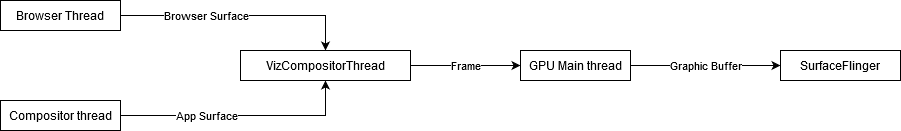
\includegraphics[width=13cm]{kththesis/Figures/surface_diagram.png}
    \caption{Overview of a frame in Chrome}
    \label{fig:surface_diagram}
\end{figure}
\paragraph{}
The Renderer surface can be computed using two different paths depending on the stages skipped: the 'Main frame' and the 'Basic Frame' in the model. The 'Main frame' is the baseline of every surface of the Renderer. However, if only a small change occurs between 2 consecutive frames for example scrolling or some CSS animations, the 'Main frame' may not need to be re-computed and is used again in the current frame. This is the 'Basic frame' path. \newline

\todo[inline]{Can these 7 steps being summarized in a figure also?}



\paragraph{}
To summarize, a frame timeline is as follows:
\begin{enumerate}
    \item The VizCompositor thread asks a new frame to the Compositor thread
    \item The Compositor thread  agrees to compute a new frame and schedules it.
    \item The Compositor might also ask for a new main frame. If so, the main thread of the Renderer referred to as Renderer thread compiles it. Regarding to the pipeline stages presented in the background, it computes the Styling, Layout, Compositing, Pre-Painting and Painting. When the Renderer thread is finished compiling the main frame, it commits it to the Compositor thread.
    \item When the Compositor receives a new main frame, it computes Tiling and Raster if necessary with the help of other threads. The main frame can then be activated: it replaces the old main frame in the memory of the Compositor thread and can be used as a baseline for future frames.
    \item Once the deadline scheduled in step 2 is up, the frame is drawn. This step is the last stage of pipeline presented previously: Drawing. The Compositor generates a ComositorFrame (cf \textit{GenerateRenderPass} and \textit{GenerateCompositorFrame}) with a main frame as a baseline and sends it to the GPU Process (cf \textit{SubmitCompositorFrame}).
    \item The VizCompositorThread receives all necessary surfaces (cf \textit{ReceiveCompositorFrame}), aggregates them into a single frame (cf \textit{SurfaceAggregation}) and sends it to CrGpuMain thread.
    \item Finally, CrGpuMain receives the frame and swap buffers for SurfaceFlinger (cf \textit{SwapBuffers} and \textit{FrameCompleted})
\end{enumerate}

However, the computation of a new Main Frame (step 3 and 4) is not always synchronized with the computation of a base frame. For example, due to various reasons \todo{Try to enumerate at least two reasons} CrRendererMain might be late in committing the main frame, and a new Basic Frame is rendered without it. Then, the Main Frame will be activated only for the following frame.

\paragraph{}
A browser frame follows a similar timeline. The main difference is that all work computed by the Compositor thread and CrRendererMain is done in the same in the same thread, CrBrowserMain. A Browser Frame always follow a path similar to a Main Frame.

\section{Comparing the Rendering Process}
   
    The background section presented an overview of Android's Garphics pipeline, with the Application Renderer itself divided into 7 stages : input handling, animation, measurement and layout, draw, sync and upload, issue commands, process and swap buffers. 
    
    It is possible to extract detailed information about an Android application frames thanks to the command \textit{adb shell dumpsys gfxinfo framestats}. This outputs multiple graphic information, such as total number of frames rendered, number of janky frames
    
    We can observe some of those stages in a Systrace recorded with the command: \textit{python systrace.py sched gfx view app -a [package-name] -o [output-file]}.
    
    \begin{figure}[!ht]
        \includegraphics[width=15cm]{kththesis/Figures/android_systrace_frame.jpg}
        \caption{Application Renderer on Android}
        \label{fig:android_systrace}
    \end{figure}
    
    
    \subsection{Chrome's pipeline}
    \todo[inline, color=cyan!20]{Describe Chrome's pipeline model and how I came up with it}
       As was described in the Background chapter, Chrome contains several processes, including the Browser Process, the Renderer and the GPU Process.
       
       To automate tracing, the Chrome Devtools Protocol was used. Its experimental domain 'Tracing' allows to record the same events as Chrome's Tracing tool. This enable the automation of both tracing and event processing to extract a model. \newline
The resulting model is presented in Figure \ref{fig:chrome_graphics_simple}. For a more detailed version with all the events tracked to know if a frame is truly rendered, see Annex \ref{?}.

To link the empirical model to the pipeline stages presented in the background, Parsing, Styling, Layout, Compositing, Pre-painting, and Painting are all computed for a 'Main frame' in the main thread of the Renderer process CrRendererMain. Tiling and Raster are also computed for a 'Main frame' but in the Compositor thread, sometimes with the help of other threads and even the GPU Process. The last step, Drawing is executed in several steps. The Compositor thread first computes a 'CompositorFrame' from the 'Main frame' available and sends to the VizCompositorThread in the GPU Process. The VizCompositorThread wait for all necessary surfaces and aggregates them, before sending them to the main thread of the GPU Process. CrGpuMain can then swap the buffers to push the frame to SurfaceFlinger. The frame is now complete.

\item The VizCompositorThread, probably because of a VSYNC event that happened previously, asks for a new frame to the Renderer process with the event 'IssueBeginframe' which contains a bind\_id.
    \item The Compositor thread of the Renderer process discard or accept it with the event 'ReceiveBeginFrame' which contains the same bind\_id. This event also call 'Scheduler::BeginFrame' which contains a sequence\_number necessary to follow the frame afterwards.
    \item The Compositor may ask a new main frame, and schedules the next step depending on the urgency of the frame with the event Scheduler::BeginImplFrame containing the same sequence\_number. The event asking for a new main frame contains a begin\_frame\_id useful to follow the frame in the thread CrRendererMain.
    \item If a new main frame was asked, it is compiled in CrRendererMain. The pipeline stages Styling, Layout, Compositing, pre-Painting and Painting are computed here if necessary.
    \item If a new main frame was committed by CrRendererMain, Tiling and Raster may be computed by the Compositor and other threads if necessary. Then, it is activated: the new main frame replaces the old one in the Compositor.
    \item The deadline of the scheduler is up: Scheduler::OnBeginImplFrameDeadline is called with the same sequence\_number as the beginning. This event itself calls several other events : GenerateRenderPass, GenerateCompositorFrame and SendCompositorFrame containing a bind\_id and LayerTreeHost::PrepareToDraw containing a SourceFrameNumber referencing the main frame used for this frame. SendCompositorFrame is not always detected but is an important event to track.
    \item The VizCompositorThread receives the CompositorFrame from the Renderer, and maybe wait for more. It then aggregates the surfaces ie the CompositorFrames into a single frame. It also assigns a put\_offset to the frame. It is not an id per say as it is not unique but the reuse of numbers are spaced enough to use it as IDs.
    \item The main thread of the GPU receives the frame and swap buffers for SurfaceFlinger. Since it is 
    
    \subsection{Method of comparison}
    \todo[inline, color=cyan!20]{Conclusions on how to compare both pipelines: a) definition of a frame b) benchmark apps used}
    
    \iffalse
    When a new surface is available, the VizCompositor thread combines it with the other surface and produces a new frame. The GPU main thread receives it and push it to SurfaceFlinger.
\paragraph{}
To summarize, a frame timeline is as follows:
\begin{enumerate}
    \item The \badge{VizCompositorThread} asks for a new frame to the Renderer process (cf \textit{IssueBeginFrame}).
    \item The Compositor thread of the Renderer process agrees to compute a new frame (cf \textit{ReceiveBeginFrame}) and schedules it (cf \textit{Scheduled}).
    \item The Compositor might also ask for a new main frame (cf \textit{SendRequestMainFrame}). If so, the main thread of the Renderer process CrRendererMain compiles it (cf \textit{BeginMainFrame}). In regards to the pipeline stages presented in the background, it computes the Styling, Layout, Compositing, Pre-Painting and Painting. When CrRendererMain is finished compiling the main frame, it commits it to the Compositor (cf \textit{BeginMainFrameCommit}).
    \item When the Compositor receives a new main frame (cf \textit{BeginCommit}), it computes Tiling and Raster if necessary with the help of other threads. The main frame can then be activated (cf \textit{ActivateLayerTree}): it replaces the old main frame in the memory of the Compositor thread and can be used as a baseline for future frames.
    \item Once the deadline scheduled in step 2 is up, the frame is drawn. This step is the last stage of pipeline presented previously: Drawing. The Compositor generates a ComositorFrame (cf \textit{GenerateRenderPass} and \textit{GenerateCompositorFrame}) with a main frame as a baseline and sends it to the GPU Process (cf \textit{SubmitCompositorFrame}).
    \item The VizCompositorThread receives all necessary surfaces (cf \textit{ReceiveCompositorFrame}), aggregates them into a single frame (cf \textit{SurfaceAggregation}) and sends it to CrGpuMain thread.
    \item Finally, CrGpuMain receives the frame and swap buffers for SurfaceFlinger (cf \textit{SwapBuffers} and \textit{FrameCompleted})
\end{enumerate}


A Main Frame starts to compute the frame at \textit{BeginMainFrame} timestamp. A Basic Frame which re-uses a previous main frame only starts computing at the beginning of 'ProxyImpl::ScheduleActionDraw' event. 

    To summarize, on one hand Android's pipeline is pretty straightforward and easy to follow : the OS sends VSync signals that depends on the device refresh rate, asking everything on the foreground to render a frame. In response, the UI thread calls Choreographer\#doFrame which handles callbacks for input and animation before doing some sizing and layout. The Choreographer then hands what it computed to the RenderThread which issues the draw commands and swap the buffers for SurfaceFlinger.


On the other hand, Chrome's pipeline is much less consistent and depends on a lot of parameters. We know that the VizCompositorThread also calls the Choreographer almost at each Vsync though it stops after the animation callbacks. As it is also the thread emitting 'IssueBeginFrame' events, those events are most likely linked, though I don't know when this IssueBeginFrame event is emitted compared to the Choreographer.

Thus, it is meaningless to compare Chrome's frames with Android's from the start of Choreographer or the start of Vsync.

Another point against doing this is the the input events. Those are always handled on Android inside the Choreographer, just before computing the frame. On Chrome, however, they are handled asynchronously and thus an input can affect a frame currently being drawn or start a new one.
\iffalse
Moreover, the input events also pose a problem. Those are always handled on Android inside the Choreographer, just before computing the frame. However they are handled asynchronously on Chrome and can even be handled in the middle of the computation of a new frame. An input event can affect a frame currently being drawn or start a new one. With this method of comparison, some of the frames on Chrome would contain input events while others would not. Thus, it is irrelevant. 
\fi
This leaves us with comparing the amount of time they spent on computing the frame. For Android, it starts with traversal, and can be accessed with the PerformTraversalStart timestamp. For Chrome, it is a little more complicated as a 'frame' for Android, that is a graphical buffer swapped for SurfaceFlinger, consists of several frames computed in parallel and combined on Chrome's Pipeline. \newline

As a Browser frame on PWA represents things usually handled by the application on Android like the scrollbar or refresh animation, and it also leads to a BufferSwap, 
For a 'Main frame', the computation starts with the \textit{BeginMainFrame} timestamp. For a 'Basic frame' which uses an old main frame as a baseline, it starts with the event 'ProxyImpl::ScheduleActionDraw'. 

For a Basic frame which reuse a Main frame already drawn, I believe the computation starts inside ProxyImpl::ScheduleActionDraw. For a basic frame with a new Main frame, it should start at 'BeginMainThreadFrame' event. 

As a Buffer swap consists of both a Basic frame and a Browser frame, and a Browser frame can trigger a Buffer swap by itself, the question is do we count them as part of the PWA's frame or not. If, as I suppose, the Browser frame displays things like the scrollbar, I believe we should count them as a PWA's frame as these displays are usually handled by the app on Android. 

Thus, the most meaningful comparison, in my opinion, is the time between the timestamps PerformTraversalStart->FrameCompleted on Android and PrepareToDraw/BeginMainThreadFrame(if new main frame)->FrameCompleted of the Compositor frame of the Browser frame on Chrome (depending which took longest for the corresponding Buffer swap).

\iffalse
\begin{enumerate}
    \item When do Chrome starts computing a Main Frame ? \newline
    As the first stages of Chrome's pipeline happens just after \textit{BeginMainFrame}, this timestamp will be considered the start of the computation for a Main Frame.
    \item When do Chrome starts computing a Basic Frame that re-uses a Main Frame ? \newline
    The only stage of Chrome's pipeline computed in a Basic Frame is Drawing, which starts at 'ProxyImpl::ScheduleActionDraw' event. Thus, it will be considered the start of the computation of a Basic Frame.
    \item Do frames which only changes the Browser surface count as frames to compare to Android application ? \newline
    The Browser surface represents on PWA what is usually also handled by the application on Android (scrollbar, refresh animation). Thus, those frames will also be compared to Android frames. 
    \item When both the Renderer surface and the Browser surface changes, what to consider the start of the frame ? \newline
    Since both Browser frames and Renderer frames are to be compared to Android, and they are pushed to SurfaceFlinger as a single frame, the start of the frame will be the start of the Browser or the Renderer frame depending on which happens the earliest. 
\end{enumerate}
\fi

\todo[inline, color=cyan!20]{Can I just erase since I don't look at graphic buffers? because it will just repeat the preceding paragraph}
Two aspects of memory will be measured to compare Native, Hybrid and Progressive Web Apps: the RAM and the memory used for graphics buffer queue. For Progressive Web Apps, those measures will be the result of the addition of the 3 processes on the foreground: the Browser, the Renderer and the GPU processes.

\fi
    
\section{Comparing CPU and Memory}
    \subsection{Android and Chrome tools}
    \todo[inline, color=cyan!20]{Describe available tools on Android and Chrome}
    \todo[inline]{Move to Background}
    \subsection{Evaluating Chrome tools}
    \todo[inline, color=cyan!20]{Describe Experiments used to compare Android and Chrome tools, and their results}
    \subsection{Evaluating Emulators}
    \todo[inline, color=cyan!20]{Explain why Emulators are no good for evaluating CPU and Memory}
\section{benchmark and protocol}

\iffalse
The smoothness metric defined previously depends in Progressive Web Apps on the rendering path taken by the frame. Thus, the benchmark application will have 2 features : one favouring Main Frames and the other favouring Basic Frames. The easiest way to trigger a Main Frame is to change the content of the screen. This can be done with a single click. A Basic Frame is basely triggered  
\fi
\subsection{script implementation}
\iffalse
We will focus on the fluidity of the apps that can be defined with Frame Per Second (FPS) rate.
Thus, we will compare the FPS rate of a Native Android Application and a Progressive Web App, as well as with a benchmark consisting of : 
    - an app displaying different image/texts every 16/17ms
    - an app with more effort on the CPU : modification of the same pictures/texts or new pictures/texts generated randomly.

\newline
\fi

We will measure FPS, CPU and Memory usage to see the impact of CPU and Memory usage in the fluidity of the app.
\newline
We will focus on the fluidity of the apps that can be defined with Frame Per Second (FPS) rate.
Thus, we will compare the FPS rate of a Native Android Application and a Progressive Web App, as well as with a benchmark consisting of : 
    - an app displaying different image/texts every 16/17ms
    - an app with more effort on the CPU : modification of the same pictures/texts or new pictures/texts generated randomly.
\newline

We will measure FPS, CPU and Memory usage to see the impact of CPU and Memory usage in the fluidity of the app.
\newline

\subsection{Emulators}
\iffalse
The results presented in Table \ref{tab:memulators_test} are the average of 110 measures.

\begin{table}[!ht]
    %\centering
    \begin{tabular}{|m{2,5cm}|m{2cm}|m{2cm}|m{2cm}||m{2cm}|m{2,5cm}|}
        \hline
         & \multicolumn{3}{c||}{Samsung S6 (API 7.0)} & \multicolumn{2}{|c|}{Samsung S5 (API 5.0)}  \\
         \hline
         Metrics & Physical device & Genymotion & Android Emulator & Physical device & Visual Studio Emulator \\
         \hline
         CPU Usage (\%) & 72 & 29 & 18 & 48 & 16 \\
         \hline
         RAM (KB) & 72 080 & 24 243 & 17 499 & 56 813 & 16 992 \\
         \hline
         Janky frames (\%) & 13 & 46 & 6 & 3 & 98 \\
         \hline
    \end{tabular}
    \caption{Emulators Tests}
    \label{tab:memulators_test}
\end{table}

\paragraph{}
The results between the physical devices and the emulators are too different to be used in future experiments. Thus, only the available Android smartphones will be used for this project: Samsung S6 (7.0), Samsung S5 (5.0) and Samsung Galaxy S (4.2)

\todo[inline, color=cyan!20]{I might be able to also use a Huawei (old phone with no card sim), depending on if it works and I have the time}   
\fi
\subsection{CPU}

\todo[inline, color=cyan!20]{Remove entirely the next paragraph ?}

\todo[inline]{Well it seems a result of your observations, I think it should not be here after all.}
However, there is a small issue with cpuinfo: the output is not always up-to-date, with sometimes a 15 min difference between the data displayed and the time it is called (it will display 'CPU usage from X ms to X ms ago'). This makes it difficult to use for automated experiments. Upon inspecting the source code\footnote{https://github.com/aosp-mirror/platform\_frameworks\_base/blob/master/services/core/java/com/android/server/am/ActivityManagerService.java} of meminfo and cpuinfo, it was found that the data saved by cpuinfo is updated each time meminfo is called. It was observed that was not always the case when 2 consecutive calls are too close to each other, but it is enough to have CPU usage from at least the last minute.

Upon inspecting Chrome Devtools and its source code\footnote{https://github.com/ChromeDevTools/devtools-frontend}, 3 possible methods of measuring CPU usage were identified:
\begin{enumerate}
    \item CPU graph displayed by Chrome Devtools Performance Panel
    \item cpuTime metric computed by Chrome Devtools for each frame
    \item CPU sampling events saved during a recording
\end{enumerate}

\paragraph{}
According to the source code of Chrome Devtools, the CPU graph is actually computed from the selftime of the functions. The selftime of the function is the amount of time it is running itself and does not wait for a function it called. Though a function usually use the CPU during its chole self-time, that is not always the case. The function can be paused for the CPU to perform other tasks for example. Thus, the CPU graph from Chrome Devtools, though a good approximation, is not accurate enough to compare the CPU usage of Android and Progressive Web applications. \newline
The cpuTime metric provided for each frame is computed similarly but its computation is limited to events related to the computation of the frame. Thus, it is also not usable as an accurate measure.

\paragraph{}
This leaves the CPU sampling events saved during a recording. CPU sampling \cite{cpu_sampling} can evaluate the CPU usage by retrieving regularly the functions currently running on the CPU. The more samples taken, the more accurate the estimation will be. This method was evaluated against the command line \textit{adb shell dumpsys cpuinfo} by measuring the CPU usage of a  Progressive Web App running on an Android emulated device with both methods (CPU sampling and dumpsys).
\color{blue}
The emulated device only had a single CPU core in case the CPU sampling only happen on the CPU cores running the app. The Progressive Web App was able to simulate different CPU workload depending on the frequency of a text changing.
\paragraph{}

\begin{figure}
    \centering
    \includegraphics[width=13cm]{kththesis/Figures/cpu_graph.JPG}
    \caption{CPU usage}
    \label{fig:cpu_usage}
\end{figure}

The results are the average of 100 measures were taken for each method and workload(see \autoref{fig:cpu_usage}). If the CPU sampling from Chrome Devtools was accurate enough, its curve would be close to the measures taken by dumpsys, though always behind as \textit{dumpsys cpuinfo} provides a maximum CPU usage of the application. This is not the case here.

\paragraph{}
Thus, the CPU usage of both Android and Progressive Web application will be measured with the command line \textit{adb shell dumpsys cpuinfo}.

\color{black}
    


\subsection{Benchmark applications}
\paragraph{}
Since a frame in a Progressive Web App can take 2 different rendering path depending on the changes occurring in the frame, at least 2 different features favouring one path or another will have to be developed. The Main Frame path is always triggered when changing some content on the screen since at least Painting is required. The Basic Frame path is favoured when scrolling a page, as the Compositor thread usually only needs to change the position of an already-painted layer against the display screen. 

The frame duration will be evaluated with a 3s recording, the memory snapshot will be executed after 10s of running a scenario in order to update the data for \textit{cpuinfo} and the CPU usage will be extracted shortly after.

\subsection{Scripts implementation}
\todo[inline]{Explain your technical contributions}
In order to remove the human interaction variable from the results, all experiments will be executed by automated scripts. All of them are available in a Git repository\footnote{TODO:git link, maybe create a clean repo with everything after}.

\chapter{Results}
\section{Smoothness performance}
\paragraph{Frame duration}
Though the Progressive Web App is never the fastest one to compute a frame, it is not always the slowest and surpasses the Native application in 3 instances: when changing a picture on Samsung S5 and Huawei P9-Lite, and when changing a text on Samsung S5.

\paragraph{Resources}

The results presented here are the average of 100 measures. In every scenario, the Native application uses less resources than the Hybrid and the PWA, both in terms of CPU and Memory usage. The performance of the Native, Hybrid and Progressive Web App differ depending on the device. \paragraph{}
In Scenario 1 (\autoref{tab:text:changing}), the Progressive Web App takes longer than the Hybrid app to compute a frame with an increase of 36\% on Samsung S6, 11\% on Samsung S5 and 139\% on Huawei. The difference is smaller between the Native application and the Progressive Web App, the latter being even faster than the Native app on Samsung S6.
%However, the Native application consumes a lot less resources than the Hybrid and the Progressive Web app, with the progressive Web App consuming slightly less CPU than the Hybrid app.

\paragraph{}
In Scenario 2 (\autoref{tab:text:scrolling}), the Native application is faster than both the Hybrid and the PWA on every device. A clear difference of performance is visible between the performance on Samsung S6 and the performance on Samsung S5 and Huawei. All apps compute a frame in 17-19ms on Samsung S6 while the Hybrid and Native app take only 3 to 7 ms on Samsung S5 and Huawei. However, the performance of the Progressive Web app does not improve this much and stays between 14 - 17 ms. 
%The Native app consumes less resources than the Hybrid and Progressive Web App, with the Hybrid consuming slightly less CPU than the Progressive Web App this time.

\paragraph{}
In Scenario 3 (\autoref{tab:picture:changing}), the Hybrid application is faster on all three devices. The Progressive Web App is faster than the Native app on two devices, Samsung S5 and Huawei, but lags behind by 20\% on Samsung S6. 
\end{document}

%Apart from \ref{scenario:picture:scrolling} and \ref{scenario:text:scrolling} where the Hybrid and PWA consumes similar amount of CPU, 
%\paragraph{}
%A third observation is the great difference between the frame duration of the PWA and the frame duration of the other mobile applications. The PWA is often 2 or three times slower than the mobile applications. The only time the PWA is faster is when scrolling pictures (\autoref{tab:picture:changing}). Then, the PWA compute new frames in 15ms while the native applications takes 17ms. However, the Hybrid application is still faster with only 7ms to compute a new frame.  

%\paragraph{}
%Lastly, though the PWA can compute new frames faster than the Native Application in \ref{scenario:picture:changing}, it is never faster than the Hybrid application and is even around 10ms slower in Scrolling Scenarios on Samsung S5 and Huawei P9-Lite. The Hybrid application is faster than the Native application on Changing content scenarios, and only falls 2 or 3ms behind the Native application in Scrolling scenarios. 

%However, the measurements for the progressive web app can be considered less accurate than the mobile applications as the browser could be performing tasks in the background unrelated to the progressive web app. The same reasoning can be applied for the memory usage. To maximize the accuracy of the results, the experiments were conducted in airplane mode without internet connection, and no other web page were opened. Nonetheless, the native application was found to be largely more efficient than the hybrid and progressive web application, both in terms of CPU and Memory usage. 

\chapter{Results}

\iffalse
\section{Research questions}
In almost every experiment, the PWA took to compute new frames and often by 2 or 3 times the amount of time it took for the Native and Hybrid App. Thus, we can conclude that Progressive Web Application are not as smooth as Mobile Applications.

\paragraph{}
The Progressive Web App consumed more memory than the Native application in every scenario, with the difference ranging from 58\% to 464\%. However, the Hybrid application consumed similar amount of memory than the PWA when changing content, and a lot more than the PWA when scrolling. Hence, though the memory performance of Progressive Web Apps do not compare to Native applications, it is similar or even better than Hybrid applications depending on the interaction.

\paragraph{}
The conclusion to the CPU usage of Mobile and Progressive Web App is similar to the memory consumption. In every scenario, the Progressive Web App consumed more CPU than the native application though the difference is not as big as the memory consumption. However, it also consumed similar amount of CPU than the Hybrid application when scrolling, and less when changing content. Thus, Progressive Web Apps can be considered better than Hybrid applications in terms of CPU usage, but worse than Native applications 
\fi

\iffalse
\section{Smoothness Performance}

To compare the smoothness performance of Native, Hybrid and Progressive Web Applications, the average frame duration as defined in \autoref{results:metric}, the CPU and the Memory usage were measured in 4 different scenarios: 
\begin{enumerate} [ref={Scenario}\xspace\arabic*]
    \item \label{scenario:text:changing} Changing a text (\autoref{tab:text:changing})
    \begin{table}[]
        \centering
        \begin{tabular}{|c|c|c|c|}
            \hline
             & Native & Hybrid & PWA \\
             \hline
            \textbf{Samsung S6} &   &   &   \\
            Frame (ms) & 16,50 & 13,46 & 27,62 \\
            CPU (\%core) & 7,97 & 59,59 & 28,28 \\
            Memory (MB) & 68 & 196 & 257 \\
            \hline   
            \textbf{Samsung S5} &   &   &   \\
            Frame (ms) & 14,38 & 10,43 & 21,99 \\
            CPU (\%core) & 3,63 & 44,89 & 15,09 \\
            Memory (MB) & 47 & 169 & 148 \\
            \hline
            \textbf{Huawei P9 Lite} &   &   &   \\
            Frame (ms) & 10,47 & 6,50 & 22,47 \\
            CPU (\%core) & 4,03 & 31,44 & 22,35 \\
            Memory (MB) & 50 & 243 & 276 \\
            \hline
        \end{tabular}
        \caption{Changing a text}
        \label{tab:text:changing}
    \end{table}

    \item \label{scenario:text:scrolling} Scrolling a text (\autoref{tab:text:scrolling})
    \begin{table}[]
        \centering
        \begin{tabular}{|c|c|c|c|}
            \hline
             & Native & Hybrid & PWA \\
             \hline
            \textbf{Samsung S6} &   &   &   \\
            Frame (ms) & 17,32 & 18,40 & 24,71 \\
            CPU (\%core) & 40,13 & 90,03 & 105,63 \\
            Memory (MB) & 77 & 377 & 179 \\
            \hline   
            \textbf{Samsung S5} &   &   &   \\
            Frame (ms) & 3,85 & 5,19 & 21,96 \\
            CPU (\%core) & 28,57 & 59,42 & 66,86 \\
            Memory (MB) & 49 & 341 & 243 \\
            \hline
            \textbf{Huawei P9 Lite} &   &   &   \\
            Frame (ms) & 4,46 & 6,81 & 22,09 \\
            CPU (\%core) & 20,18 & 73,55 & 105,33 \\
            Memory (MB) & 55 & 406 & 149 \\
            \hline
        \end{tabular}
        \caption{Scrolling a text}
        \label{tab:text:scrolling}
    \end{table}
    \item \label{scenario:picture:changing} Changing a picture (\autoref{tab:picture:changing})
    \begin{table}[]
        \centering
        \begin{tabular}{|c|c|c|c|}
            \hline
             & Native & Hybrid & PWA \\
             \hline
            \textbf{Samsung S6} &   &   &   \\
            Frame (ms) & 9,66 & 9,48 & 17,86 \\
            CPU (\%core) & 9,09 & 57,82 & 25,66 \\
            Memory (MB) & 87 & 300 & 349 \\
            \hline   
            \textbf{Samsung S5} &   &   &   \\
            Frame (ms) & 17,04 & 7,83 & 15,67 \\
            CPU (\%core) & 8,41 & 44,36 & 11,56 \\
            Memory (MB) & 56 & 265 & 193 \\
            \hline
            \textbf{Huawei P9 Lite} &   &   &   \\
            Frame (ms) & 10,07 & 4,83 & 13,07 \\
            CPU (\%core) & 8,99 & 32,09 & 19,36 \\
            Memory (MB) & 56 & 317 & 316 \\
            \hline
        \end{tabular}
        \caption{Changing a picture}
        \label{tab:picture:changing}
    \end{table}
    \item \label{scenario:picture:scrolling} Scrolling pictures (\autoref{tab:picture:Scrolling})
    \begin{table}[]
        \centering
        \begin{tabular}{|c|c|c|c|}
            \hline
             & Native & Hybrid & PWA \\
             \hline
            \textbf{Samsung S6} &   &   &   \\
            Frame (ms) & 13,36 & 17,44 & 24,31 \\
            CPU (\%core) & 34 & 106,68 & 102,65 \\
            Memory (MB) & 106 & 578 & 182 \\
            \hline   
            \textbf{Samsung S5} &   &   &   \\
            Frame (ms) & 3,38 & 4,62 & 21,31 \\
            CPU (\%core) & 37,21 & 60,35 & 66,35 \\
            Memory (MB) & 104 & 283 & 243 \\
            \hline
            \textbf{Huawei P9 Lite} &   &   &   \\
            Frame (ms) & 4,57 & 7,63 & 22,31 \\
            CPU (\%core) & 51,13 & 116,37 & 119,17 \\
            Memory (MB) & 97 & 614 & 154 \\
            \hline
        \end{tabular}
        \caption{Scrolling pictures}
        \label{tab:picture:Scrolling}
    \end{table}
\end{enumerate}

First, we will mention some issues that were raised during and after the experiments. Then, we will present several observations that can be made from result. \newline

\subsection{Experiment notes}
The results presented here are the average of 100 measures. However, some small issues were raised during and after the experiments.\newline
Firstly, the scrolling experiments were not as consistent between frameworks and devices as changing content was. The same drag event did not trigger the same scrolling speed, and the length of the scrolling page was different. The tools used to simulate drag events also behaved  differently. Thus, the drag events were adapted to the device and framework so that the view scrolled all the way down and a little up during the experiments. \newline
Lastly, the clocks of different threads in Chrome were sometimes found to be slightly out of sync. Thus, some events were detected before their triggering events on another thread. However, those incidents concerned events not counted in the frame duration. They were scarce and the delay was of small magnitude. Thus, it was concluded that they did not impact the results presented here.

\subsection{Takeaways}
\label{results:performance}
The first observation is the difference of frame computation time of the same application between devices. In both Scrolling scenarios (\autoref{tab:picture:Scrolling} \autoref{tab:text:scrolling}), the Native and Hybrid applications takes 3 or 4 times more time to compute a frame on Samsung S6 than on Samsung S5 and Huawei. The difference is less significant on Changing Scenarios though a two-times magnitude difference can still be observed. PWAs also offer a more consistent smoothness over devices.
\paragraph{}
The second observation concerns only the Progressive Web App. With the metric defined in \autoref{results:metric}, it was expected that scrolling would result in smaller frame computation times for PWA. This is true when displaying text though the difference is small, but not at all when displaying pictures. 

\paragraph{}
The third observation concerns the memory used by the applications. The Native application consumes significantly less CPU and Memory than the Hybrid and Progressive Web Application in every scenario. On the one hand, the Native application consumes only around 50 MB of RAM, 100 MB at most when scrolling pictures. On the other hand, the PWA and Hybrid app consumes at least 150 MB of RAM and even up to 600 MB for the Hybrid application.

\paragraph{}
The difference of CPU consumption is not as big as the memory performance, but still significant with a 2 times magnitude difference between the Native and the Hybrid and PWA, sometimes more. The Hybrid application consumes slightly less CPU than the PWA during scrolling, while the PWA consumes less CPU than the Hybrid app when changing content. 

\paragraph{}
The last observation is a comparison of the Native and Hybrid applications. The performance of the Hybrid application is better when changing content while the Native application is better when scrolling. However, the Hybrid application only follows it by 2 or 3ms during a scroll, while the Native application can lag behind the Hybrid app by up to 10 ms. 


\fi
\chapter{Discussion}

This may be due to the size of the frameworks used for the Hybrid and PWA, while the framework used in Native application is part of the OS and not the application.

However, it should be noted that the scrolling experiments were not as consistent between devices and frameworks than when changing content. The same drag event did not trigger the same scrolling speed across device and framework, and the length of the scrolling page was different. It is also difficult to simulate the same drag event with \textit{monkeyrunner} and the Input Domain of Chrome DevTools Protocol. More experiments would be needed to confirm the performance observed when scrolling. Moreover, the clocks of different threads in Chrome were found to be slightly out of sync. Thus, some events were detected before their triggering events on another thread. However, those incidents concerned events not counted in the frame duration. They were scarce and of small magnitude and thus do not invalidate the results presented previously.

\todo{Each RQ as a section non in question form}

\paragraph{R1: How can we compare the smoothness of Progressive Web Apps and Mobile Applications?}
To answer this question, a model of Chrome's rendering pipeline was empirically built and compared to Android's rendering pipeline. It was found that comparing frames as defined by either Android or Chrome was irrelevant since their rendering pipeline was too different. Instead, the amount of time it takes to compute a frame and push it to SurfaceFlinger was used. \newline
However, this metric was identified only for Progressive Web Application running on Chrome browser on Android. Other popular browsers and other OS must be studied in order to reach a real conclusion, for example the Safari browser on iOS. This metric might be used with other browsers as well, but a study of its rendering pipeline will be needed to confirm its relevance and identify when the browser starts computing a frame. This can be a suggestion for future work related to the smoothness of Progressive Web Application. 

\paragraph{R2: With the metrics identified previously, are Progressive Web Applications as smooth as Mobile Applications?}
Though the Progressive Web App was found to be faster than the Native application in some cases, it was more often the slowest out the three applications by up to a 10ms margin. The Hybrid application, which was the fastest app or the second fastest by only 2 or 3ms seems a better cross-platform solution for mobile applications. \newline
However, it should be noted that the scrolling experiments were not as consistent between devices and frameworks than when changing content. The same drag event did not trigger the same scrolling speed across device and framework, and the length of the scrolling page was also different. Moreover, it is difficult to simulate the same drag event with \textit{monkeyrunner} and the Input Domain of Chrome DevTools Protocol. More experiments would be needed to confirm the performance observed when scrolling.

\paragraph{R3: How many resources are used to render a smooth application?}
The amount of resources used differ greatly between the frameworks. The Native application was in all scenarios the one consuming the less resources by far. The Hybrid application was slightly more efficient than the PWA for scrolling content, and slightly less efficient when changing content. Though this result might contradict the study done by Kerssens \cite{PWAapplicability}, it concurs with the results found by Ciman and Gaggi \cite{ciman2017empirical} who found that cross-platform applications consumes more energy than native applications, especially when updating User Interface elements. This may be due to the additional layer present in the Hybrid and PWA and necessary to run the application.
\fi

\chapter{Conclusion}

One possibility of future work identified in the limitations is the extension of this thesis to other browsers and OS, especially iOS which is often discarded in academic research about Progressive Web Apps. This study can also be extended with other cross-platform and Web framework, for example Xamarin and Angular.\newline
The other possibilities involve studying another aspect of performance of a mobile application, for example its responsiveness, its battery consumption or the performance of other animations like videos or those found in games.
